\section{Моделирование и оптимизация однокубитных логических операций}
\label{sec:chapter_3}

\subsection{Двухфотонные рамановские переходы}

Опишем кратко принцип работы двухфотонного рамановского возбуждения, подробный вывод можно найти в книге \cite{Steck}. Рассмотрим трёхуровневую систему в $\Lambda$-схеме (рис. \ref{fig:raman_scheme}). Гамильтониан такой системы во вращающейся системе отсчета и приближении вращающейся волны имеет вид

\begin{equation}
	H = H_{A} + H_{AF} + H_{F},
\end{equation}

где $H_{A}$ - гамильтониан атома, $H_{AF}$ - гамильтониан взаимодействия атома с полем. Гамильтониан поля $H_{F}$ можно считать константой, так как поле содержит огромное число степеней свободы, считается классическим, из-за чего динамика атома никак на него не влияет. 

\begin{equation}
	H_{A} = \frac{p^2}{2m} + \hbar \Delta_0 \ket{0}\bra{0} + \hbar \Delta_{1}\ket{1}\bra{1},
\end{equation}

\begin{equation}
	H_{AF} = \frac{\hbar}{2}\left(\Omega_0\ket{0}\bra{e}e^{-i\vec{k}_0\vec{r}}+\Omega_0^*\ket{e}\bra{0}e^{i\vec{k}_0\vec{r}}\right) + \frac{\hbar }{2}\left(\Omega_1\ket{1}\bra{e}e^{-i\vec{k}_1\vec{r}}+\Omega_1^*\ket{e}\bra{1}e^{i\vec{k}_1\vec{r}} \right).
\end{equation}

\begin{figure}[H]
	\centering
	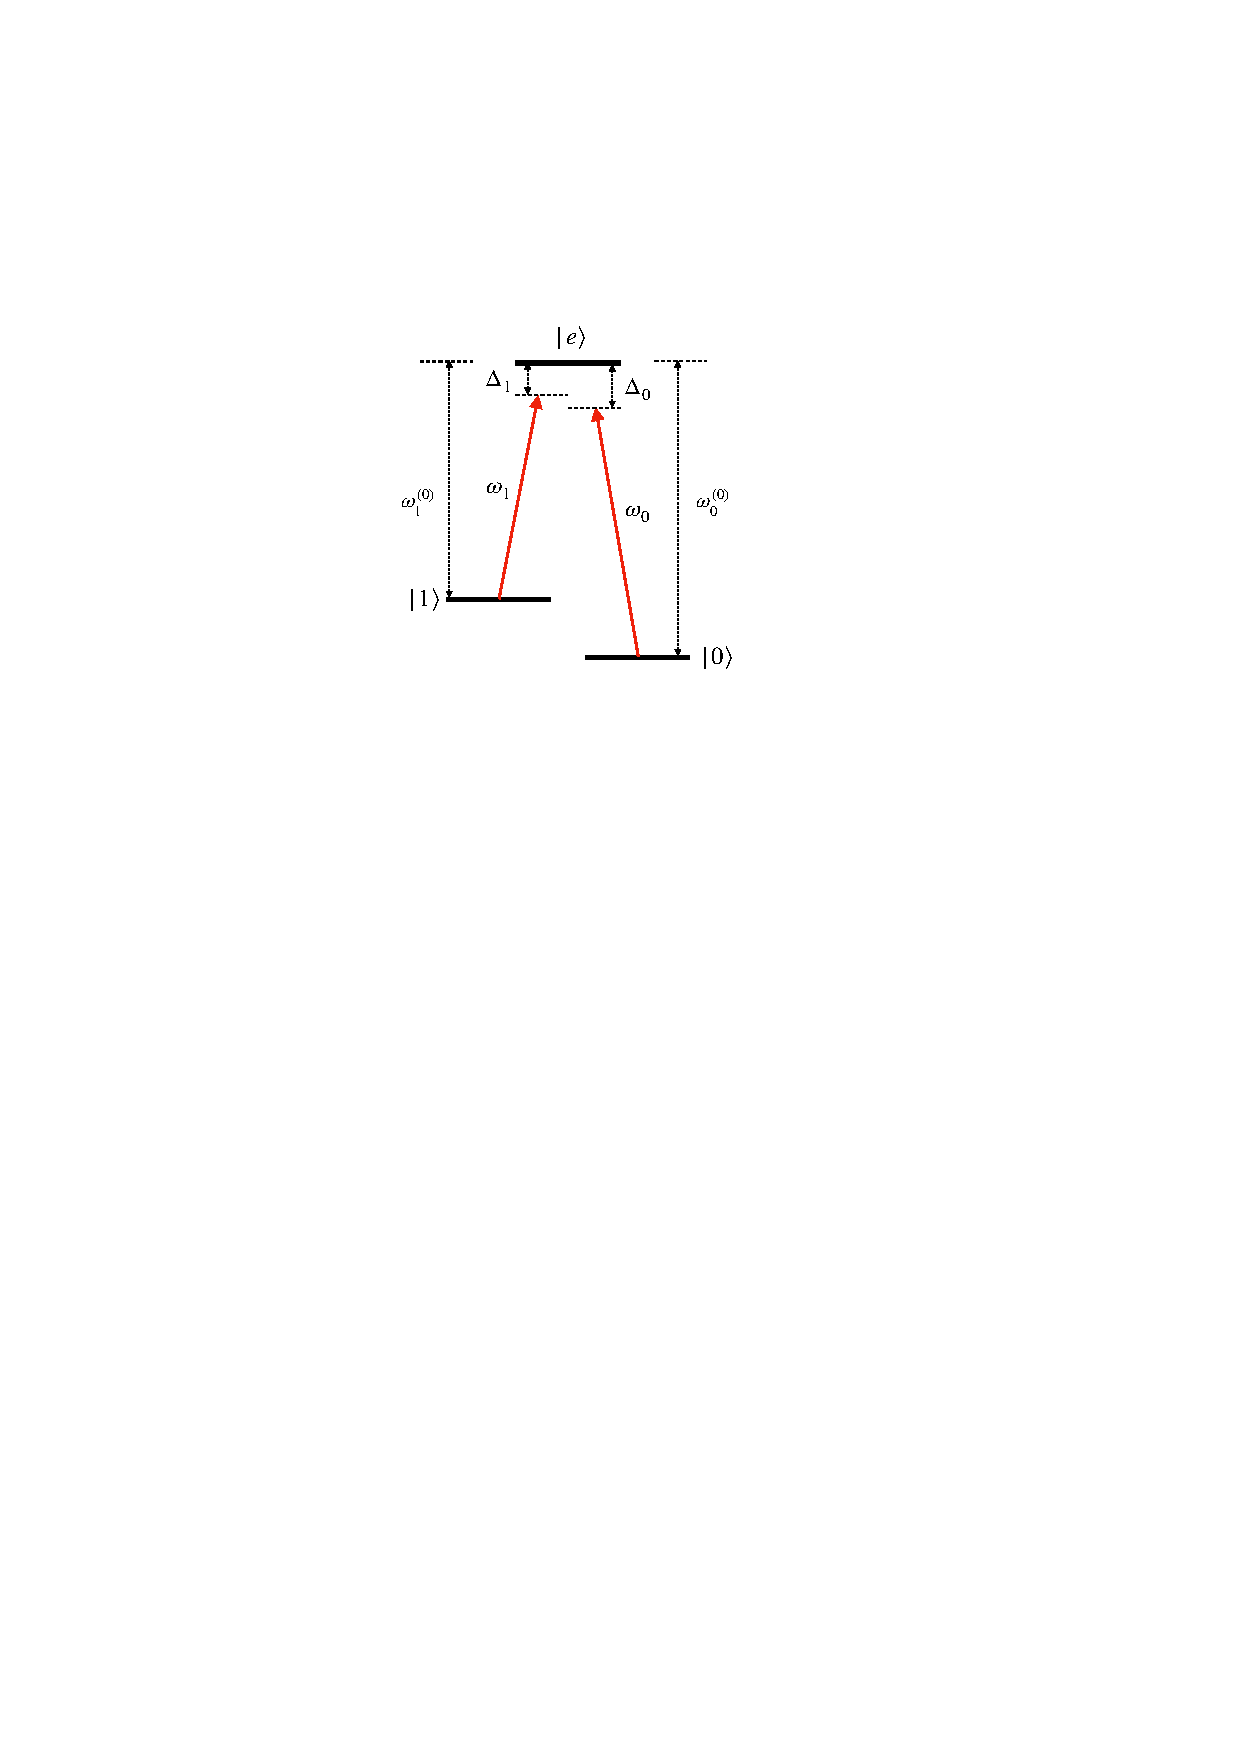
\includegraphics[width=0.5\textwidth]{images/raman_scheme.pdf}
	\caption{Трёхуровневая система в $\Lambda$-конфигурации.}
	\label{fig:raman_scheme}
\end{figure}

Сдвинем все энергии на $\Delta=\frac{\Delta_0+\Delta_1}{2}$, запишем систему дифференциальных уравнений на коэффициенты разложения по базису трёхуровневой системы

\begin{equation}
	\begin{cases}
		\left|\psi\right\rangle=\psi_0\ket{0}+\psi_1\ket{1}+\psi_e\ket{e},	\\

		i\hbar\partial_t\psi_e=\frac{p^2}{2m}\psi_e+\frac{\hbar\Omega_0^*}{2}e^{i\vec{k}_0\vec{r}}\psi_0+\frac{\hbar\Omega_1^*}{2}e^{i\vec{k}_1\vec{r}}\psi_1-\hbar\Delta\psi_e,	\\

		i\hbar\partial_t\psi_0=\frac{p^2}{2m}\psi_0+\frac{\hbar\Omega_0}{2}e^{-i\vec{k}_0\vec{r}}\psi_e+\hbar\left(\Delta_0-\Delta\right)\psi_0, \\

		i\hbar\ \partial_t\psi_1=\frac{p^2}{2m}\psi_1+\frac{\hbar\Omega_1}{2}e^{-i\vec{k}_1\vec{r}}\psi_e+\hbar\left(\Delta_1-\Delta\right)\psi_1.
	\end{cases}
\end{equation}

Нам интересна динамика на временах много меньших, чем скорость спонтанного распада из промежуточного состояния, поэтому промежуточный уровень $\ket{e}$ можно адиабатически исключить, положив $\partial_t\psi_e=0$. Также будем пренебрегать кинетической энергией атома, считая  $\frac{p^2}{2m}\ll\hbar\Delta$. В итоге из первого уравнения системы получим выражение для коэффициента разложения $\psi_e$

\begin{equation}
	\psi_e=\frac{\Omega_0^*}{2\Delta}e^{i\vec{k}_0\vec{r}}\psi_0+\frac{\Omega_1^*}{2\Delta}e^{i\vec{k}_1\vec{r}}\psi_1.
	\label{eq:psie}
\end{equation}

Подставим это соотношение в уравнения на $\psi_0, \psi_1$, получим 

\begin{equation}
	\begin{cases}
		i\hbar \partial_t\psi_{0} = \frac{p^2}{2m}\psi_{0} + \hbar(\Delta_0 + \omega_{AC_0})\psi_{0} + \frac{\hbar \Omega_{R}^*}{2}e^{i(\vec{k}_1-\vec{k}_0)\vec{r}}\psi_{1},\\
		i\hbar \partial_t\psi_{1} = \frac{p^2}{2m}\psi_{1} + \hbar(\Delta_1 + \omega_{AC_1})\psi_{1} + \frac{\hbar \Omega_{R}}{2}e^{-i(\vec{k}_1-\vec{k}_0)\vec{r}}\psi_{0},
	\end{cases}
\end{equation}

где двуфхотонная частота Раби

\begin{equation}
	\Omega_{R} = \frac{\Omega_0^* \Omega_1}{2\Delta}
\end{equation}

и штарковские сдвиги

\begin{equation}
	\omega_{AC_i} = \frac{|\Omega_{i}|^2}{4\Delta}.
\end{equation}

Учитывая зависимость от импульса и что $\exp(-i\vec{k}\vec{r})\ket{\vec{p}} = \ket{\vec{p}-\hbar \vec{k}}$, получаем уравнения

\begin{equation}
	\begin{cases}
		i\hbar \partial_t \psi_{0}(\vec{p}) = \left(\frac{p^2}{2m} + \hbar \Delta_{0} + \hbar \Omega_{AC_0}\right) \psi_{0}(\vec{p}) + \frac{\hbar \Omega_{R}}{2}\psi_{1}(\vec{p} + 2\hbar \delta\vec{k}), \\
		i\hbar \partial_t \psi_{1}(\vec{p}+2\hbar \delta\vec{k}) = \left(\frac{p^2}{2m} + \hbar \Delta_{1} + \hbar \Omega_{AC_1}\right) \psi_{1}(\vec{p}+2\hbar \delta\vec{k}) + \frac{\hbar \Omega_{R}^*}{2}\psi_{0}(\vec{p}).
	\end{cases}
\end{equation}

Отсюда получаем эффективный гамильтониан двухуровневой системы ($\hbar=1$) $\ket{0}, \; \ket{1}$

\begin{equation}
	H_R = \frac{\Delta_R}{2}\sigma_{z} + \frac{\text{Re }\Omega_{R}}{2}\sigma_{x} + \frac{\text{Im }\Omega_{R}}{2}\sigma_{y},
\end{equation}
\begin{equation}
	\Delta_{R} = -4\omega_{R}\left(\frac{p_{\parallel}+\hbar \delta k}{\hbar \delta k}\right) + (\Delta_0 - \Delta_1) + (\omega_{AC_0} - \omega_{AC_1}), \; \hbar\omega_{R} = \frac{\hbar^2 \delta k ^2}{2m},
\end{equation}

где $\hbar\omega_R = \frac{\hbar^2 \delta k^2}{2m}$ - энергия отдачи, $p_{\parallel}$ - импульс вдоль направления $\delta \vec{k}$. 


Из соотношения \ref{eq:psie} также можно получить оценку на скорость спонтанного распада как

\begin{equation}
	\begin{aligned}
		& R=\Gamma\rho_{ee}=\Gamma\left|\psi_e\right|^2=\frac{\Gamma|\Omega_0|^2}{4\Delta^2}\rho_{00}+\frac{\Gamma|\Omega_1|^2}{4\Delta^2}\rho_{11}+\\
& +\frac{\Gamma}{4\Delta^2}\left(\Omega_0\Omega_1^*e^{i\left(\vec{k}_1-\vec{k}_0\right)\vec{r}}\rho_{01}+\Omega_0^*\Omega_1e^{-i\left(\vec{k}_1-\vec{k}_0\right)\vec{r}}\rho_{10}\right).
	\end{aligned}
	\label{eq:scattering_rate}
\end{equation}

Для нашего эксперимента с очень хорошей точностью выполняется $\Omega_0=\Omega_1=\Omega,\; \vec{k}_0=\vec{k}_1$. Остаётся понять, что происходит с когерентностями $\rho_{01},\; \rho_{10}$. Ясно, что когерентности будут содержать зависимость от времени на двухфотонной частоте Раби. Усредним скорость распада по периоду осцилляций Раби, тогда когерентности уйдут. С учётом $\rho_{00}+\rho_{11}\simeq 1$ для большой отстройки от промежуточного состояния, получаем оценку на скорость распада

\begin{equation}
	R=\frac{\Gamma|\Omega|^2}{4\Delta^2}.
	\label{eq:decay_rate}
\end{equation}



\subsection{Моделирование точности рамановских операций}

\subsubsection{Спонтанный распад из промежуточного состояния}
\label{sec:spontaneous}

Будем использовать скорость спонтанного распада для оценки ошибки из-за распада из промежуточного состояния. Так как в нашей системе спонтанный распад происходит не только на кубитные состояния $\ket{0}, \; \ket{1}$, но и на соседние сверхтонкие подуровни, то более честно было бы учитывать распад отдельно в кубитные состояния и оставшиеся подуровни сверхтонкого расщепления основного состояния. Однако, для расчета ошибки по такой схеме требуется численно моделировать систему дифференциальных уравнений с двумя сильно отличающимися характерными частотами - двухфотонной частотой Раби и отстройкой от промежуточного состояния. Такие вычисления занимают очень много времени, а хочется получить лишь оценку ошибки из-за спонтанного распада, поэтому кажется разумным ограничиться формулой \ref{eq:decay_rate}. Посчитаем ошибку из-за спонтанного распада от радиуса перетяжки рамановского лазера и отстройки от промежуточного состояния. Мощность лазера, то есть однофотонные частоты Раби, будем считать фиксированной. При реализации однокубитного гейта одиночным импульсом ошибка из-за спонтанного распада равна 

\begin{equation}
	(1-F)_{sp}=\frac{1}{2}\frac{R}{\Omega_{R}} = \frac{\Gamma}{4\Delta}.
\end{equation}

Для отстройки от промежуточного состояния $\Delta = 2\pi \times 50 \text{ ГГц}$ и ширины линии $\Gamma = 2\pi \times 6 \text{ МГц}$ \cite{Rb87} промежуточного уровня $5^2P_{1/2}$ получаем значение ошибки $(1-F)_{sp} = 3 \times 10^{-5}$, то есть на текущий момент точность однокубитных рамановских операций не ограничивается спонтанным распадом из промежуточного состояния, им можно пренебречь.

\subsubsection{Тепловое движение атома в оптическом пинцете}
\label{sec:monte_carlo}

Рассмотрим атом в оптическом пинцете, образованном гауссовым пучком с амплитудой поля и интенсивностью

\begin{equation}
	E=E_0\left(\frac{w\left(z\right)}{w_0}\right)\exp\left(-\frac{x^2+y^2}{w\left(z\right)^2}\right)\exp{\left(-i\left(kz+k\frac{r^2}{2R\left(z\right)}-\psi\left(z\right)\right)\right)},    
\end{equation}

\begin{equation}
	I=I_0\left(\frac{w\left(z\right)}{w_0}\right)^2\exp\left(-\frac{{2(x}^2+y^2)}{w\left(z\right)^2}\right),
\end{equation}

где параметры гауссового пучка определяются как

\begin{equation}
	w\left(z\right)=w_0\sqrt{1+\left(z/z_0\right)^2},
\end{equation}

\begin{equation}
	R\left(z\right)=z\left(1+\left(z_0/z\right)^2\right),
\end{equation}

\begin{equation}
	\psi\left(z\right)=\arctan\left(z/z_0\right),
\end{equation}

\begin{equation}
	z_0=\frac{\pi w_0^2}{\lambda}.
\end{equation}

Здесь $E_0$, $I_0$ – амплитуда и интенсивность в центре гауссового пучка, $w_0$ – радиус перетяжки гауссового пучка, $w\left(z\right)$ - радиус перетяжки от расстояния до центра ловушки вдоль $z$, $\psi\left(z\right)$ - набег фазы, $R\left(z\right)$ - кривизна волнового фронта, $z_0$ – длина Рэлея, которая определяется радиусом перетяжки и длиной волны излучения. Гауссов пучок формирует дипольную ловушку, потенциал атома в которой задается формулами \cite{grimm1999optical}

\begin{equation}
	U\left(x,y,z\right)=U_0\left(1-\left(\frac{w\left(z\right)}{w_0}\right)^2\exp{\left(-\frac{2\left(x^2+y^2\right)}{w\left(z\right)^2}\right)}\right),	
\end{equation}

\begin{equation}
	U_0 = \frac{\hbar \Gamma^2 I_0}{8 I_{sat}\Delta}.
\end{equation}

Здесь $U_0$ - потенциал в центре оптической ловушки, который зависит от ширины линии возбуждённого состояния $\Gamma$, отстройки от возбужденного состояния $\Delta$ и интенсивности в центре гауссова пучка $I_0$, $I_{sat}$ - интенсивность насыщения. При $\Delta > 0$ потенциал является притягивающим (красные ловушки), при $\Delta < 0$ отталкивающим (синие ловушки). В моделировании рассматривается красная ловушка с фиксированной отстройкой и интенсивностью в центре. Энергия атома в оптическом пинцете в таком случае равна 

\begin{equation}
	E\left(\vec{r},\vec{v}\right)=U\left(x,y,z\right)+\frac{m\left(v_x^2+v_y^2+v_z^2\right)}{2}.
\end{equation}	 

Считая что атом имеет распределение Больцмана по энергиям с некоторой температурой $T$, можно записать плотность вероятности атома находиться в состоянии $(x,y,z,v_x,v_y,v_z) = (\vec{r},\vec{v})$ как 

\begin{equation}
	\rho\left(\vec{r},\vec{v}\right)\sim \exp{\left(\frac{-E\left(\vec{r},\vec{v}\right)}{kT}\right)}.
\end{equation}

Потенциал оптической ловушки также можно приблизить гармоническим потенциалом, получить радиальную и продольную частоты колебаний:

\begin{equation}
	\omega_r=\sqrt{\frac{4U_0}{mw_0^2}},
\end{equation}

\begin{equation}
	\omega_z=\sqrt{\frac{2U_0}{mz_0^2}}.
\end{equation}

В дальнейшем это будет важно для измерения размеров ловушки по параметрическому нагреву атома.
 	   	 
Зная совместное распределение атома по координатам и скоростям, можно произвести сэмплирование реализаций атома в оптической ловушке, например, с помощью алгоритма Метрополиса-Гастингса, одного из методов Markov Chain Monte-Carlo (MCMC). После сэмплирования можно будет рассчитать осцилляции Раби для каждой отдельной реализации атома в оптическом пинцете, затем усреднить и получить модель сигнала осцилляций из эксперимента. Алгоритм Метрополиса-Гастингса для сэмплирования реализаций атома в оптическом пинцете состоит из следущих шагов:

\begin{enumerate}
	\item Задать начальные значения координат и скоростей $\left(\vec{r}_0,\vec{v}_0\right)$. Далее будем вектор координат и скоростей на i-ой итерации алгоритма обозначать ${\vec{\xi}}^{\left(i\right)}$

	\item С помощью пробного распределения с плотностью вероятности $q\left(\vec{\xi}\right)$ сгенерировать смещение $d\vec{\xi}$.

	\item Посчитать значение $a=\frac{p\left({\vec{\xi}}^{\left(i\right)}+d\vec{\xi}\right)}{p\left({\vec{\xi}}^{\left(i\right)}\right)}\frac{q\left({\vec{\xi}}^{\left(i\right)}|{\vec{\xi}}^{\left(i\right)}+d\vec{\xi}\right)}{q\left({\vec{\xi}}^{\left(i\right)}+d\vec{\xi}|{\vec{\xi}}^{\left(i\right)}\right)}$. Для симметричных распределений $a=\frac{p\left({\vec{\xi}}^{\left(i\right)}+d\vec{\xi}\right)}{p\left({\vec{\xi}}^{\left(i\right)}\right)}$.

	\item Сгенерировать значение u из равномерного распределения на отрезке $\left[0,1\right]$. Если $a>u$, то ${\vec{\xi}}^{\left(i+1\right)}={\vec{\xi}}^{\left(i\right)}$, иначе точка отклоняется.

	\item Вернуться к шагу $2$.
\end{enumerate}

В качестве пробного распределения для Метрополиса-Гастингса возьмём многомерное нормальное распределение с диагональной матрицей ковариаций

\begin{equation}
	\sqrt{\frac{kT}{m}}\text{diag}\left(1/\omega_r,1/\omega_r, 1/\omega_z, 1, 1, 1\right).
\end{equation}

Элементы матрицы ковариации учитывают характерные значения координаты и скорости для атома в оптическом пинцете при заданной температуре и параметрах ловушки. $\omega_r,\omega_z$ – колебательные частоты ловушки. Пример сэмплирования показан на рисунке 2. Видно, что в случае глубокого потенциала ловушки/ низкой температуры атома распределение по координатам и скоростям совпадают с гармоническим. 
Для расчёта точности квантовых операций можно ограничиться динамикой атома в гармоническом потенциале, так как в ангармоническом режиме (мелкая ловушка/ горячий атом) точность гейтов заведомо будет низкой из-за эффекта Доплера и разброса атома по координате. Точное сэмплирование в потенциале оптического пинцета остаётся актуальным для определения температуры по эксперименту release and recapture \cite{Tuchendler2008EnergyDA}, про который будет рассказано далее. 

\begin{figure}[H]
	\centering
	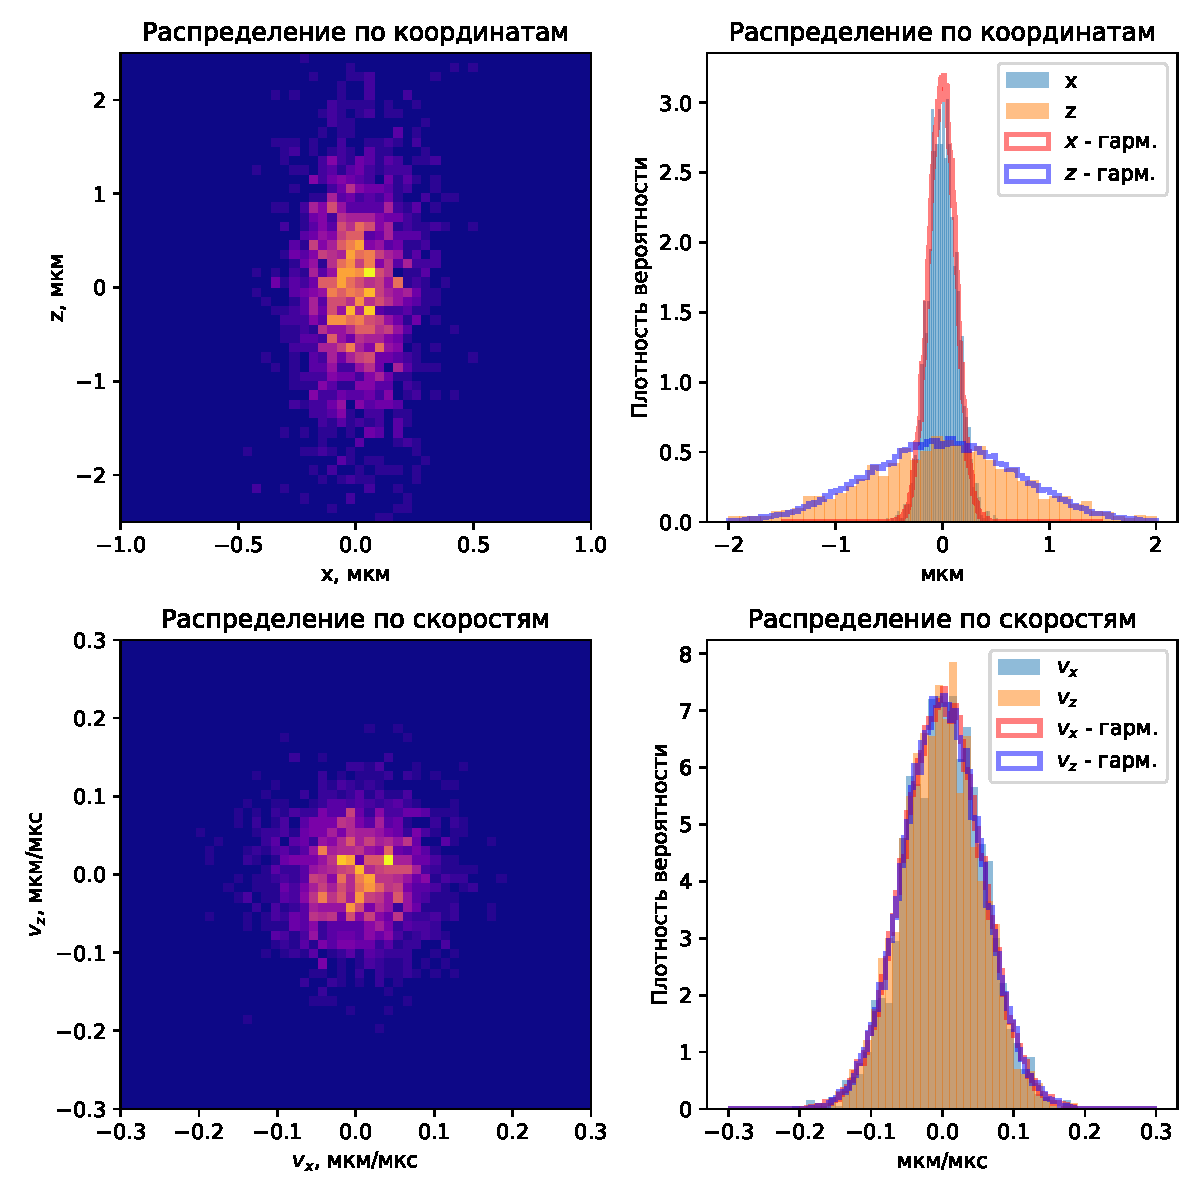
\includegraphics[width=0.6\textwidth]{images/mcmc.pdf}
	\caption{Полученные распределения атома по энергиям, координатам и скоростям для глубокой ловушки. Сравнение с гармоническим приближением.}
	\label{fig:mcmc_samples}
\end{figure}

Для уменьшения корреляции между сэмплами нужно прореживать выборку и выбрасывать первые точки, чтобы марковская цепь сошлась к нужному распределению. Для больших выборок прореживание не существенно, но для небольшого числа точек ($\sim 100$) это нужно делать.

Динамика атома в оптическом пинцете приводит к нескольким механизмам декогеренции: выход из двухфотонного резонанса из-за эффекта Доплера, флуктуации частоты атома из-за разброса атома по координатам. В моделировании эти процессы учитываются так:

\begin{enumerate}
	\item С помощью Монте-Карло сэмплируются начальные координаты и скорости атома, которые далее используются как начальные условия.

	\item Из выборки берётся точка $\xi^{(i)} = \left(x^{\left(i\right)},y^{\left(i\right)},z^{\left(i\right)},{v_x}^{\left(i\right)},{v_y}^{\left(i\right)},{v_z}^{\left(i\right)}\right)$, траектории атома считаются в гармоническом приближении:

	\begin{itemize}
		\item $x\left(t\right)=x^{\left(i\right)}\cos{\left(\omega_rt\right)}+\frac{v_x^{\left(i\right)}}{\omega_r}\sin{\left(\omega_rt\right)}$,

		\item $y\left(t\right)=y^{\left(i\right)}\cos{\left(\omega_rt\right)}+\frac{v_y^{\left(i\right)}}{\omega_r}\sin{\left(\omega_rt\right)}$,

		\item $z\left(t\right)=z^{\left(i\right)}\cos{\left(\omega_zt\right)}+\frac{v_z^{\left(i\right)}}{\omega_z}\sin{\left(\omega_zt\right)}$.
	\end{itemize}

	\item Частота Раби (амплитуда + фаза) рамановского лазера $\Omega_{R}$ пропорциональна интенсивности лазера $I_{R}$. Эффект Доплера вносит сдвиг в отстройку от промежуточного уровня $\Delta$, отстройка от двухфотонного резонанса компенсируется за счёт сонаправленной конфигурации пучков. Так как отстройка от промежуточного уровня составляет порядка $50 \text{ ГГц}$, то эффектом Доплера можно пренебречь. После подстановки траекторий атома в оптическом пинцете двухфотонная частота Раби начинает зависеть от времени:

	\begin{itemize}
		\item $\Omega_{R}(t) = \Omega_{R}^{(0)} \frac{I_{R}(\vec{r}(t))}{I_{R}(0)}$. 
	\end{itemize}	
\end{enumerate}
	
Далее динамика системы с гамильтонианом, зависящим от времени, считается численно с помощью пакета \href{https://www.qojulia.org/}{QuantumOptics.jl} \cite{kramer2018quantumoptics}, получившиеся матрицы плотности\footnote{Хотя в моделировании решается уравнение Шрёдингера, усреднять нужно именно матрицы плотности, так как векторы состояния определены с точностью до глобальной фазы. Разная глобальная фаза у векторов состояния может появиться, например, при учёте в моделировании фазовых шумов лазера. }усредняются по траекториям атома. В результате моделирования нам бы хотелось найти значения отстройки от промежуточного состояния и радиуса перетяжки, которые дают наименьшую ошибку однокубитной операции. Ясно, что при увеличении радиуса перетяжки точность операции будет расти, так как будет пропадать зависимость частоты Раби от температуры. Однако, также будет расти кроссток на соседних кубитах, так как рамановский лазер будет частично попадать на них и возбуждать осцилляции Раби. Чтобы найти оптимальные параметры эксперимента, будем считать суммарную ошибку из-за теплового движения и кросстока. Также учтём ошибку из-за спонтанного распада. Результаты моделирования для разных мощностей лазера показаны на рисунке \ref{fig:simple_pulse_errors}. Мощность лазера фиксируется заданием двухфотонной частоты Раби $\Omega^*$ для радиуса перетяжки рамановскго лазера $w_R = 2.5\text{ мкм}$ и отстройке от промежуточного состояния $\Delta = 2\pi \times 50 \text{ ГГц}$.

\begin{figure}[H]
	\centering
	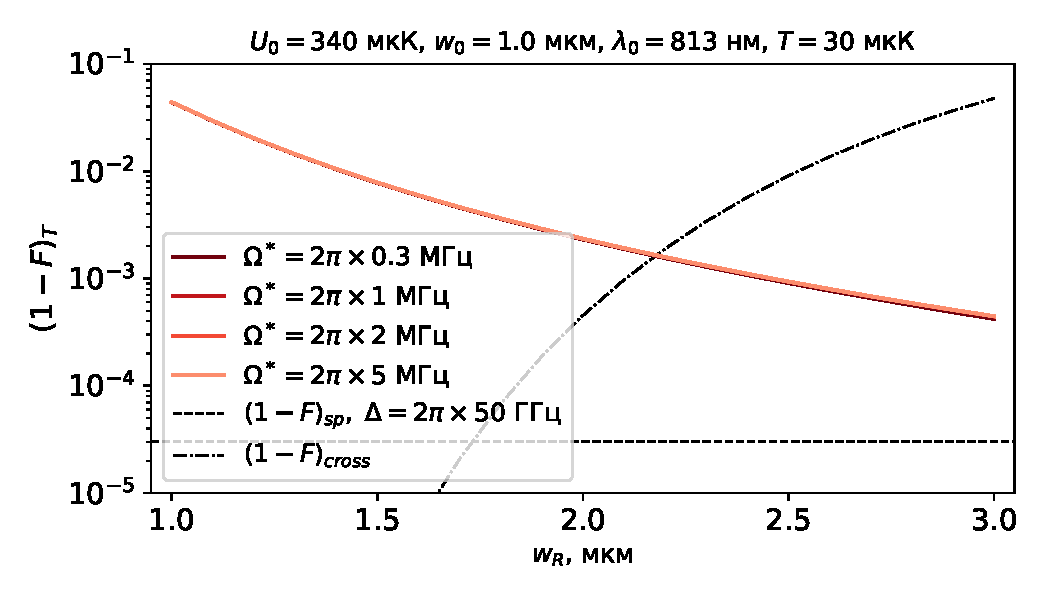
\includegraphics[width=0.48\textwidth]{images/simple_Omega.pdf}
	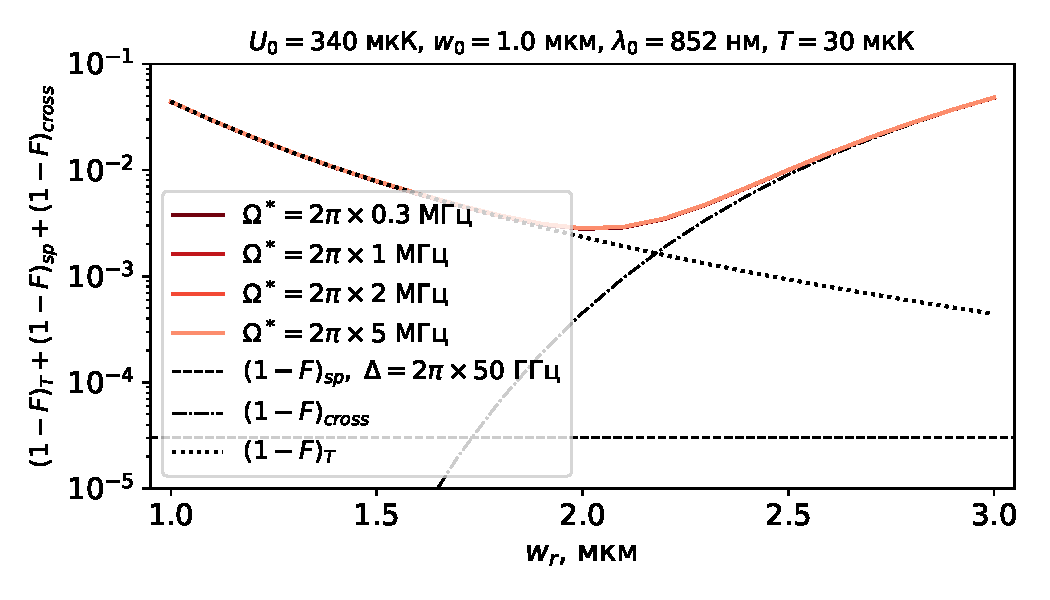
\includegraphics[width=0.48\textwidth]{images/simple_Omega_total.pdf}
	\caption{Слева: ошибка из-за теплового движения для обычного $\pi$-импульса. Справа: суммарная ошибка из-за теплового движения, кросс-тока и спонтанного распада для обычного $\pi$-импульса.}
	\label{fig:simple_pulse_errors}
\end{figure}

Видно, что ошибка определяется тепловым движением атома в оптическом пинцете, оптимальное значение радиуса перетяжки с учётом кросс-тока составляет $w_{R} = 2.0\text{ мкм}$, значение ошибки $\pi$-импульса составляет $3 \cdot 10^{-3}$.

На рисунке \ref{fig:rabi_sample} приведён пример осцилляций Раби между кубитными состояниями с рамановским двухфотонным возбуждением для разных радиусов перетяжки рамановского лазера $w_R$. 

\begin{figure}[H]
	\centering
	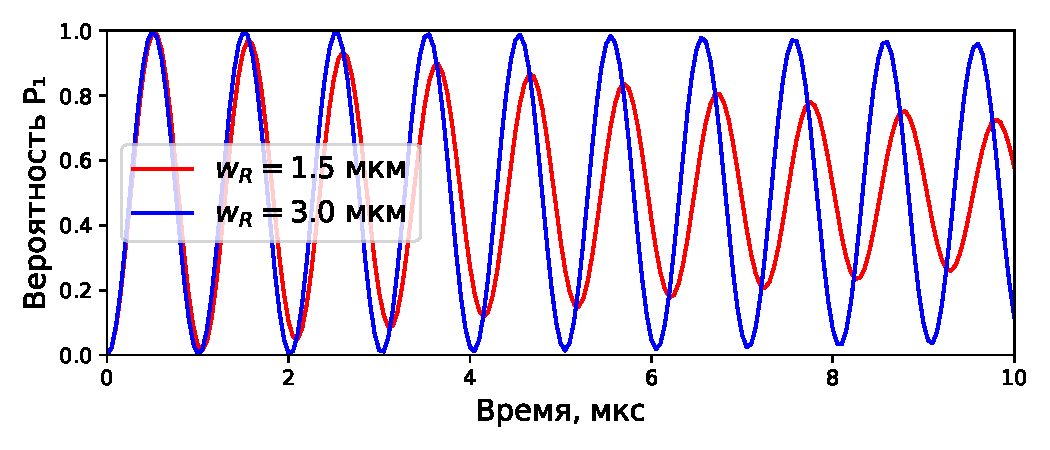
\includegraphics[width=0.65\textwidth]{images/rabi_sample.pdf}
	\caption{Осцилляции Раби между кубитными состояниями с рамановским двухфотонным возбуждением. Осцилляции с меньшим радиусом перетяжки рамановского лазера затухают быстрее за счёт большего влияния теплового движения атома.}
	\label{fig:rabi_sample}
\end{figure}

Видно, что для радиуса перетяжки рамановского лазера $w_R = 1.5 \text{ мкм}$ осцилляции Раби затухают значительно быстрее, чем для $w_R = 3.0\text{ мкм}$. Остальные параметры соответсвуют экспериментальным значениям $U_0 = 340\text{ мкК}, \; T = 30\text{ мкК}, \; w_0 = 1.0\text{ мкм}, \; \lambda_0 = 813\text{ нм}, \; \lambda_{R} = 795 \text{ нм}$. Быстрое затухание при маленьких соотношениях радиусов перетяжки рамановского лазера и оптического пинцета $w_R/w_0$ связано с тем, что для таких параметров двухфотонная частота Раби $\Omega_{R}(\vec{r}) \sim I(\vec{r})$ сильно изменяется при небольшом отклонении атома от центра ловушки. Это приводит к тому, что разные атомы осциллируют на немного разных частотах Раби, при усреднении осцилляций Раби по реализациям атома в оптическом пинцете фактически складываются синусы с разными частотами, что ведёт к затуханию. Ситуация с затуханием осцилляций Раби из-за теплового движения атома очень похожа на ситуацию со сбоем фазы немонохроматичного источника, для которого также можно ввести время когерентности. Особенно понятной эта связь становится, если рассмотреть предельный случай большой частоты Раби $\Omega_{R} \gg \omega_r, \omega_z$ (по сравнению с частотами колебаний атома в ловушке). В этом пределе атомы можно считать неподвижными во время осцилляций Раби, получить ``немонохроматический источник'' с частотой $\Omega_{R}$, имеющей распределение показанное на рисунке \ref{fig:non_monochromatic}.

\begin{figure}[H]
	\centering
	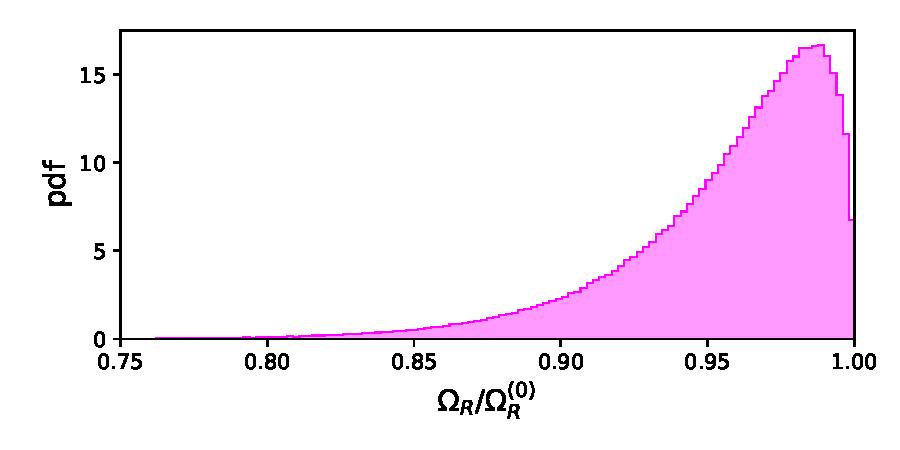
\includegraphics[width=0.75\textwidth]{images/non_monochromatic.pdf}
	\caption{Пример распределения частот Раби для характерных экспериментальных параметров.}
	\label{fig:non_monochromatic}
\end{figure}

По аналогии с временем когерентности для немонохроматического источника можно посчитать характерное время затухания из-за теплового движения атома. Рассмотрим для простоты двумерный случай когда атом движется только в радиальном направлении, покоится по оси $z$. Характерная координата атома в гармоническом приближении оценивается как

\begin{equation}
	r_c^2=\left< r^2\right> = \int_{\mathbb{R}^2} \rho(r)r^2 d\vec{r}^2 = \frac{2kT}{m\omega_r^2} = \frac{1}{2}\frac{kT}{U_0}w_0^2,
\end{equation}

а характерная частота Раби как

\begin{equation}
	\Omega_{c} = \Omega_0 \exp\left(-\frac{2r^2_c}{w_R^2}\right)=\Omega_0 \exp\left(-\frac{kT}{U_0}\frac{w_0^2}{w_R^2}\right).
\end{equation}

Отсюда получаем время сбоя фазы как 

\begin{equation}
	(\Omega_0 - \Omega_c)\tau_{r} = \Omega_0 \tau\left[1 - \exp\left(-\frac{kT}{U_0}\frac{w_0^2}{w_R^2}\right)\right] \simeq \Omega_0 \tau_r \frac{kT}{U_0}\left(\frac{w_0}{w_R}\right)^2 \sim 2\pi,
\end{equation}

то есть отношение характерного времени затухания к периоду осцилляций Раби $T_{R}$ равно

\begin{equation}
	\tau_{r}/T_{R} \sim \frac{U_0}{kT}\left(\frac{w_R}{w_0}\right)^2.
\end{equation}

Аналогичные выкладки можно провести для колебаний вдоль оси $z$, положив $r=0$. Получится следующее соотношение

\begin{equation}
	\tau_{z}/T_{R} \sim \frac{U_0}{kT}\left(\frac{z_{R}}{z_{0}}\right)^2 \sim \frac{U_0}{kT}\left(\frac{w_{R}}{w_{0}}\right)^4 \left(\frac{\lambda_{0}}{\lambda_{R}}\right)^2 \sim \frac{U_0}{kT}\left(\frac{w_{R}}{w_{0}}\right)^4.
\end{equation}

Так как для характерных параметров эксперимента $w_{R}/w_{0} \sim 1-6$, то для характерного времени затухания выполняется $\tau^{-1} = \tau_{r}^{-1} + \tau_{z}^{-1} \sim \tau_{r}^{-1}$. Окончательно получаем оценку на неточность однокубитной операции ($\pi$-импульс) из-за тепловго движения\footnote{Здесь $(1-F)_{T}$ следует воспринимать как единый символ. Под $F$ понимается fidelity операции, индекс $T$ напоминает происхождение ошибки - конечная температура атома $T$.}

\begin{equation}
	(1-F)_{T} \sim \frac{kT}{U_0}\left(\frac{w_0}{w_R}\right)^2.
\end{equation}

Из этой оценки можно сделать важный вывод: при характерных соотношениях экспериментальных параметров $U_0/kT \sim 10, \; w_R /w_0 \sim 1-6$ ошибка однокубитной операции составляет порядка $10^{-2}-10^{-1}$, что достаточно много. Фактически это означает, что для реализации точных $(1-F)_{T} < 10^{-3}$ локальных $w_{R} \sim w_0$ однокубитных операций с рамановским двухфотонным возбуждением требуется охлаждать атом до температур порядка $U_0/kT \sim 1000$, то есть $T \sim 1\text{ мкК}$ при глубине ловушки $U_0 = 1000 \text{ мкК}$. Для сравнения квант колебаний вдоль радиального направления при соответствующих параметрах эксперимента имеет температуру порядка $5 \text{ мкК}$. Это означает, что для достижения такой точности операций требуется либо охлаждать атом до основного колебательного состояния, что можно сделать с помощью метода Resolved-sideband Raman cooling \cite{Kaufman_2012,Thompson_2013}, либо искать какие-то другие подходы к реализации однокубитных операций с рамановским двухфотонным возбуждением.

Так как конфигурация нашей установки не позволяет реализовать такой тип охлаждения, то были рассмотрены альтернативные способы реализации однокубитных операций с рамановским возбуждением осцилляций Раби. При реализации однокубитных локальных операций с помощью flat-top пучков \cite{Gillen_Christandl_2016} возникает проблема с масштабируемостью, так как flat-top пучки сильно чувствительны к аберрациям \cite{Zupancic:16,Ebadi_2021} при жёсткой фокусировке на атом. Это проблема усугубляется тем, что для выполнения локальных операций требуется отклонять пучки с помощью АОД, что может усиливать аберрации. Далее в этой главе будет рассмотрена замена обычных импульсов последовательностью импульсов BB1, устойчивой к отклонениям частоты Раби от идеального значения. 

Ещё одним возможным вариантом является увеличение расстояния между атомами с $3\text{ мкм}$ до $10-20\text{ мкм}$. В таком случае появится возможность делать рамановское возбуждение с соотношением перетяжек $w_{R}/w_{0} \sim 10$ без увеличения кросстока между соседними кубитами. Требуемое соотношение температур при этом смягчается до $U_0/kT \sim 100$, что уже можно достичь, например, с помощью метода охлаждения Polarization gradient cooling \cite{PhysRevA.96.033406}. Однако, такой подход усложняет выполнение двухкубитных операций за счёт уменьшения энергии ридберговской блокады, требует использовать зонную архитектуру квантового процессора \cite{Bluvstein:2024aa}, при которой двухкубитные операции выполняются в отдельной зоне вакуумной камеры. Такое большое расстояние между соседними кубитами также усложняет адресацию лазерных пучков на атомы, находящиеся ближе к краю массива, так как эффективность диффракции на АОДе падает с увеличением угла отклонения лазерного луча. Подводя итог, такой подход не кажется перспективным.

\subsection{Измерение параметров модели}

\subsubsection{Глубина оптической ловушки}
\label{sec:trap_depth}

Для дипольной ловушки с большой красной отстройкой (FORT) глубина потенциала совпадает с оптическим штарковским сдвигом $\Delta_{AC}$ \cite{grimm1999optical}, т.е. можно измерить глубину напрямую. Для измерения штарковского сдвига можно приготовить атом в состоянии $\ket{0}$, посветить на него полем с отстройкой $\Delta$ от номинального перехода и частотой Раби $\Omega$ в течение некоторого времени $\tau$, а дальше измерить населённость состояния $\ket{1}$. Пользуясь общим видом оператора эволюции \ref{eq:evolution_operator}, получим выражение для измеряемой населенности состояния $\ket{1}$

\begin{equation}
	\left|\bra{1}U(\tau)\ket{0}\right|^2 = \sin^2\left(\frac{\sqrt{\Omega^2+(\Delta+\Delta_{AC})^2}\tau}{2}\right)\frac{1}{1+((\Delta+\Delta_{AC})/\Omega)^2}.
	\label{eq:Stark_measure}
\end{equation}

Огибающая этой функции это лоренцовский контур от отстройки $\Delta$ с шириной порядка частоты Раби $\Omega$ и центром в $\Delta = -\Delta_{AC}$. Если мы знаем резонансную частоту перехода в отсутствие штарковского сдвига от ловушки, то можно по измерениям населенности состояния $\ket{1}$ его измерить. Измерения стоит проводить при маленькой частоте Раби и большой длительности импульса, тогда получится измерить штарковский сдвиг с наибольшей точностью. 

\begin{figure}[H]
	\centering
	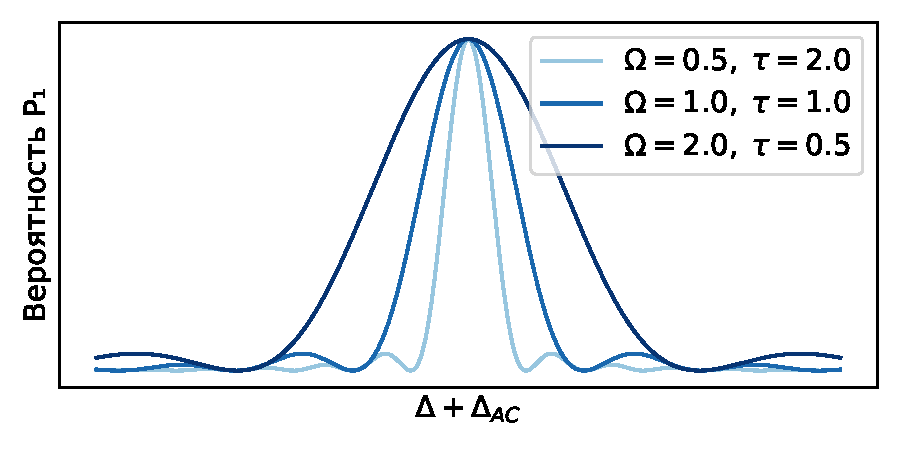
\includegraphics[width=0.6\textwidth]{images/Stark_measure_drawing.pdf}
	\caption{Графики по формуле \ref{eq:Stark_measure} для разных соотношений частоты Раби и времени измерения при фиксированном $\Omega\tau = 1$. Видно, что измерения с маленькой частотой Раби и большой длительностью получаются точнее.}
	\label{fig:Stark_drawing}
\end{figure}

Так как для измерения состояния атома используется дополнительный пучок push-out, то необходимо также учитывать штарковский сдвиг от него. Чтобы измерить сдвиг только от ловушки, можно провести два эксперимента: сначала измерить суммарный штарковский сдвиг, а затем мигать пучками ловушки trap и выбивающего пучка push-out в разные моменты времени. Схема измерения оптического штарковсого сдвига с мигающими пучками показана на рисунке \ref{fig:Stark_measure_scheme}.

\begin{figure}[H]
	\centering
	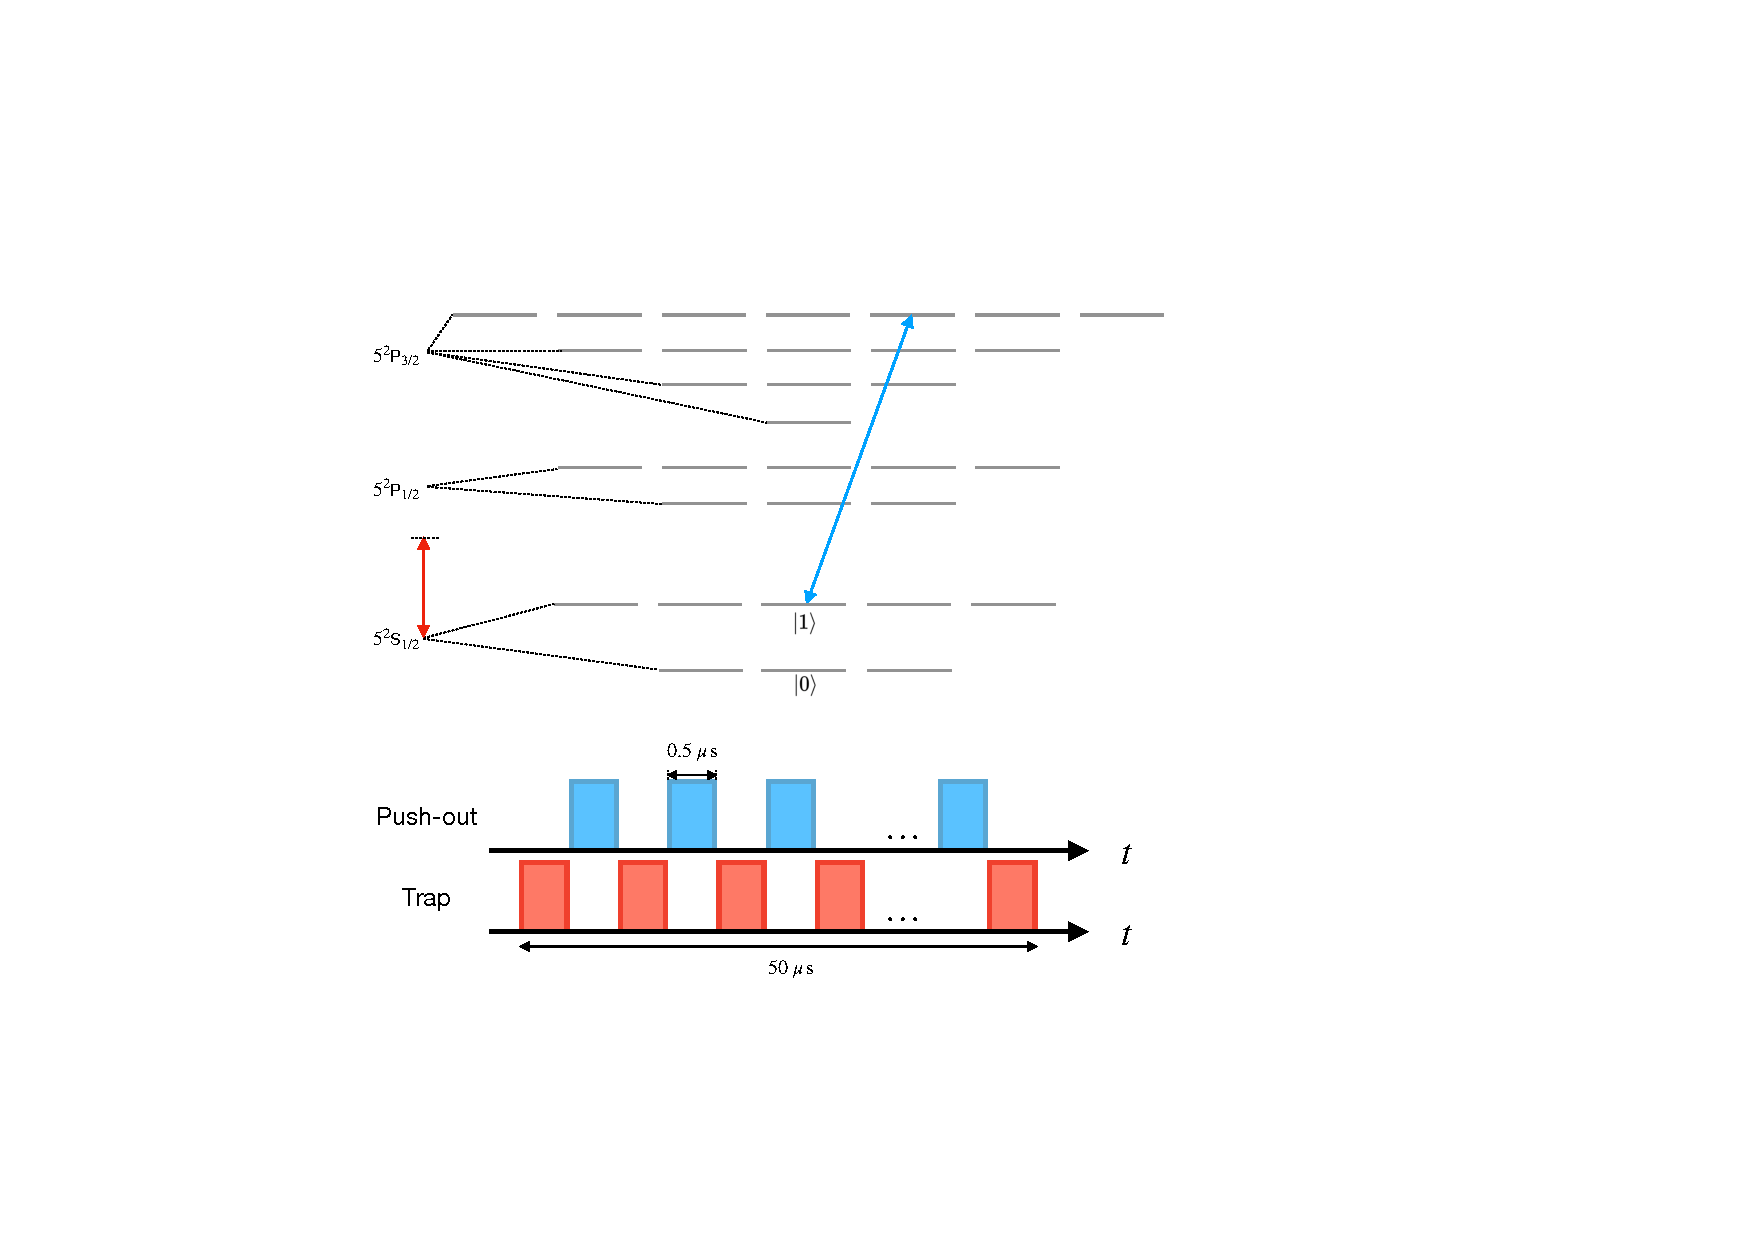
\includegraphics[width=0.7\textwidth]{images/measurement.pdf}
	\caption{Схема измерения оптического штарковского сдвига от дипольной ловушки с мигающими пучками.}
	\label{fig:Stark_measure_scheme}
\end{figure}

Результаты измерения оптического штарковского сдвига представлены на рисунке \ref{fig:trap_depth}. Глубина ловушки составляет $U_0 = 340 \text{ мкК}$.

\begin{figure}[H]
	\centering
	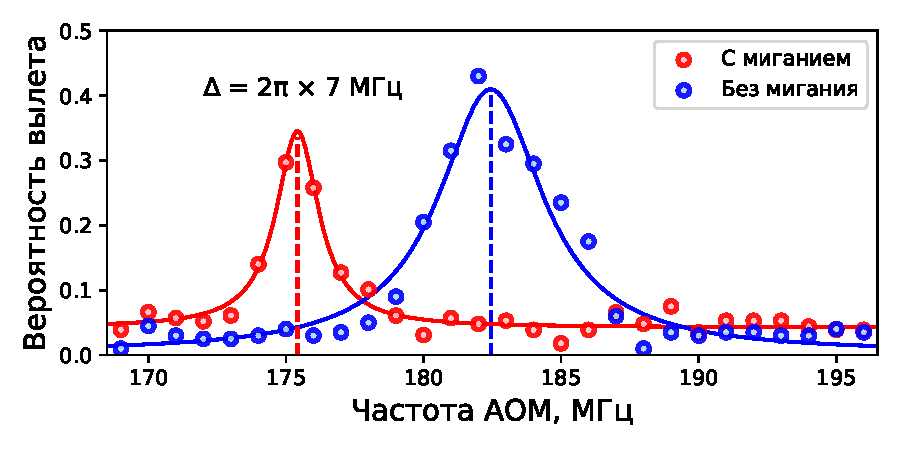
\includegraphics[width=0.6\textwidth]{images/trap_depth.pdf}
	\caption{Измерение оптического штарковского сдвига от дипольной ловушки с и без мигания ловушкой. Разница между центрами резонансов равна оптическому штарковскому сдвигу от дипольной ловушки.}
	\label{fig:trap_depth}
\end{figure}

\subsubsection{Геометрические параметры ловушки, параметрический нагрев}
\label{sec:trap_geom}

Так как оптические пинцеты сформированы жёстко сфокусированными гауссовыми пучками с маленьким радиусом перетяжки, то непосредственное измерение геометрических размеров ловушки по камере затруднительно. По этой причине радиус перетяжки оптического пинцета измеряется по параметрическому нагреву атома \cite{Param_Heating_Friebel,Param_Heating_Savard,Param_Heating_Gardiner,J_uregui_2001}. Альтернативным способом измерения геометрических параметров оптического пинцета является измерение колебательных частот ловушки в эксперименте Resolved-sideband Raman cooling \cite{Kaufman_2012,Thompson_2013}, однако он не реализован на нашей установке. 

\begin{figure}[H]
	\centering
	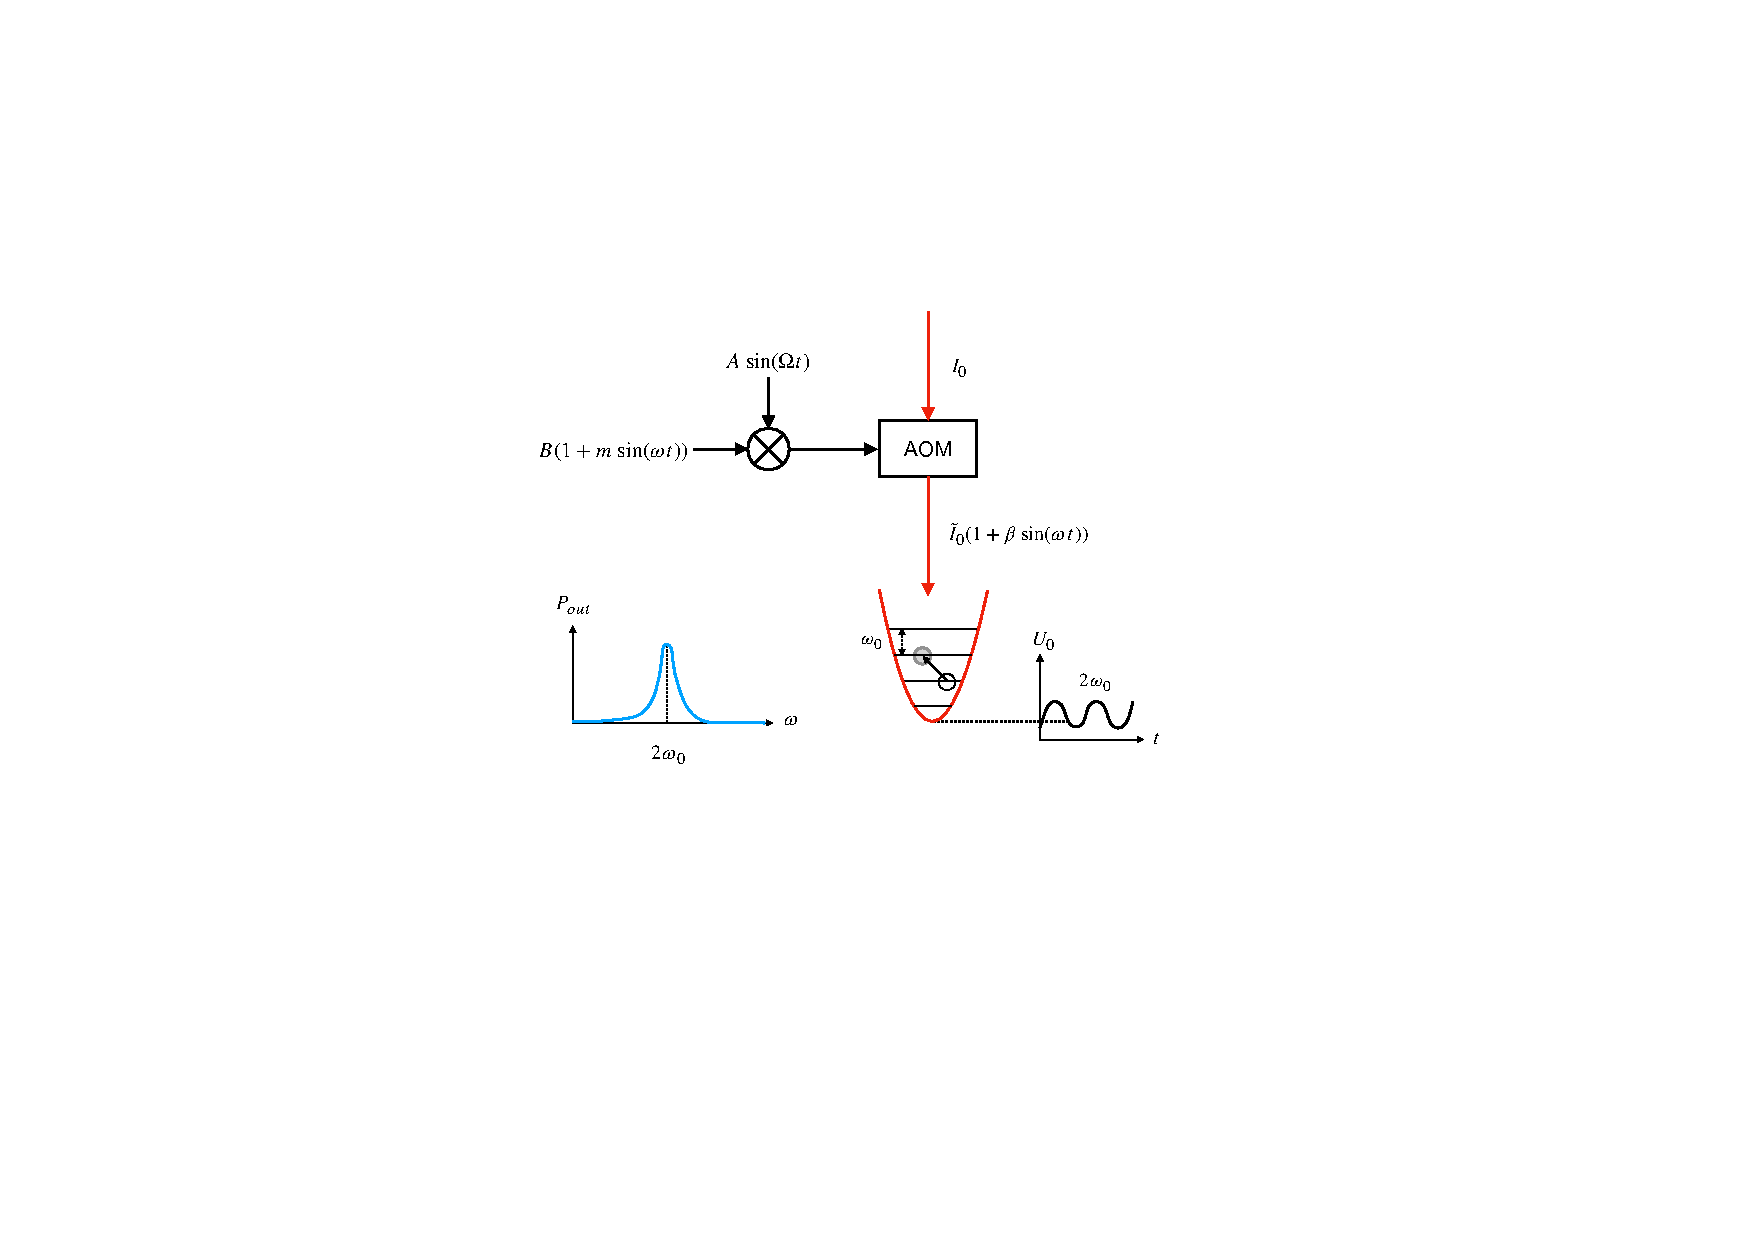
\includegraphics[width=0.7\textwidth]{images/parametric_heating.pdf}
	\caption{Принципиальная схема измерения колебательных частот: несущий сигнал смешивается с модулирующим, что приводит к модуляции эффективности дифракции луча ловушки на АОМе, из-за чего модулируется глубина ловушки.}
	\label{fig:parametric_heating}
\end{figure}

Суть метода состоит в том, что при модуляции глубины потенциала оптической ловушки $\tilde{U}_0(t) = U_0 (1 + m \sin(\omega t))$ на удвоенной частоте собственных колебаний $\omega = 2\omega_r, 2\omega_z$ атом испытывает параметрический резонанс \cite{LL_mechanics}, нагревается и вылетает из ловушки. Таким образом, в зависимости вероятности вылета атома из ловушки от частоты модуляции $\omega$ будут наблюдаться резонансы на удвоенных частотах собственных колебаний, из которых можно посчитать радиус перетяжки $w_0$ и длину Рэлея $z_0$. Принципиальная схема измерений показана на рисунке \ref{fig:parametric_heating}. Модуляция частоты, подающейся на АОМ, приводит к модуляции эффективности дифракции, что в свою очередь приводит к модуляции интенсивности лазера, который создаёт оптические ловушки. Ширина параметрических резонансов определяется глубиной модуляции, поэтому измерения лучше проводить при малой глубине модуляциии и большом времени раскачки. Результаты измерений представлены на рисунке \ref{fig:oscillation_frequencies}. 

\begin{figure}[H]
	\centering
	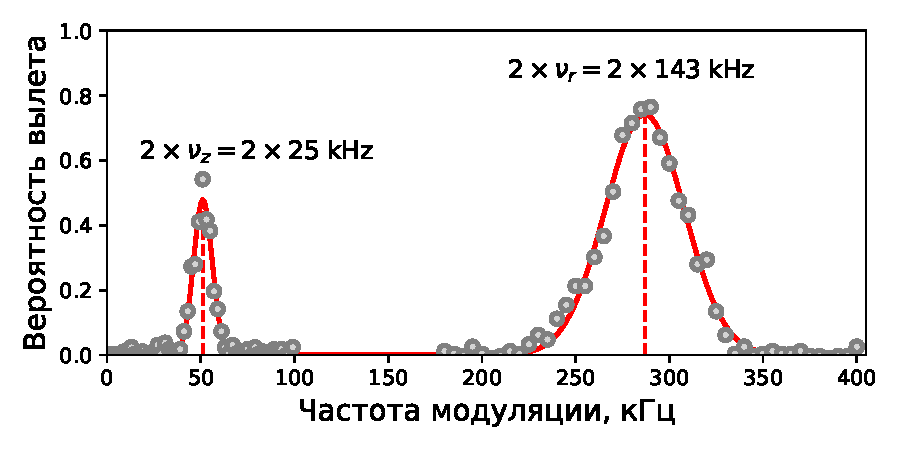
\includegraphics[width=0.7\textwidth]{images/oscillation_frequencies.pdf}
	\caption{Параметрические резонансы в вероятности вылета атома из оптической ловушки при модуляции глубины ловушки.}
	\label{fig:oscillation_frequencies}
\end{figure}

Стоит отметить, что в обычном режиме работы оптического пинцета сигнал модуляции $(1+m\sin(\omega t))$ не смешивается с сигналом несущей, которая далее подаётся на АОМ. Из-за этого глубина ловушки $U_0$ с и без умножителя могут отличаться, что приведет к изменению колебательных частот ловушки. Из-за этого для расчёта геометрических параметров ловушки следует пользоваться следующим соотношением

\begin{equation}
	w_0 = \frac{\lambda_0}{\sqrt{2}\pi}\frac{\omega_r}{\omega_z}.
	\label{eq:w0}
\end{equation}

Формула \ref{eq:w0} не зависит от глубины ловушки, поэтому ей можно пользоваться даже с учётом отличия глубины ловушки при измерениях геометрических параметров от её значения во время выполнения логических операций. Отсюда получаются геометрические параметры ловушки $w_0 = 1.1 \text{ мкм}, \; z_0 = 4.2 \text{ мкм}$. Стоит отметить, что форма линии параметрических резонансов асимметрична, что связано с ангармонизмом потенциала, формируемого гауссовым пучком \cite{Param_Heating_Friebel,J_uregui_2001}. Центр резонансов отличается от ожидаемого значения $2\omega$ и смещён примерно на $(1.6-1.7)\omega$, как это следует из моделирования (рис. \ref{fig:parametric_test}). В связи с этим стоит ещё раз отметить преимущество формулы \ref{eq:w0} - она зависит лишь от отношения колебательных частот, сдвиг центров резонансов на неё не влияет.

\begin{figure}[H]
	\centering
	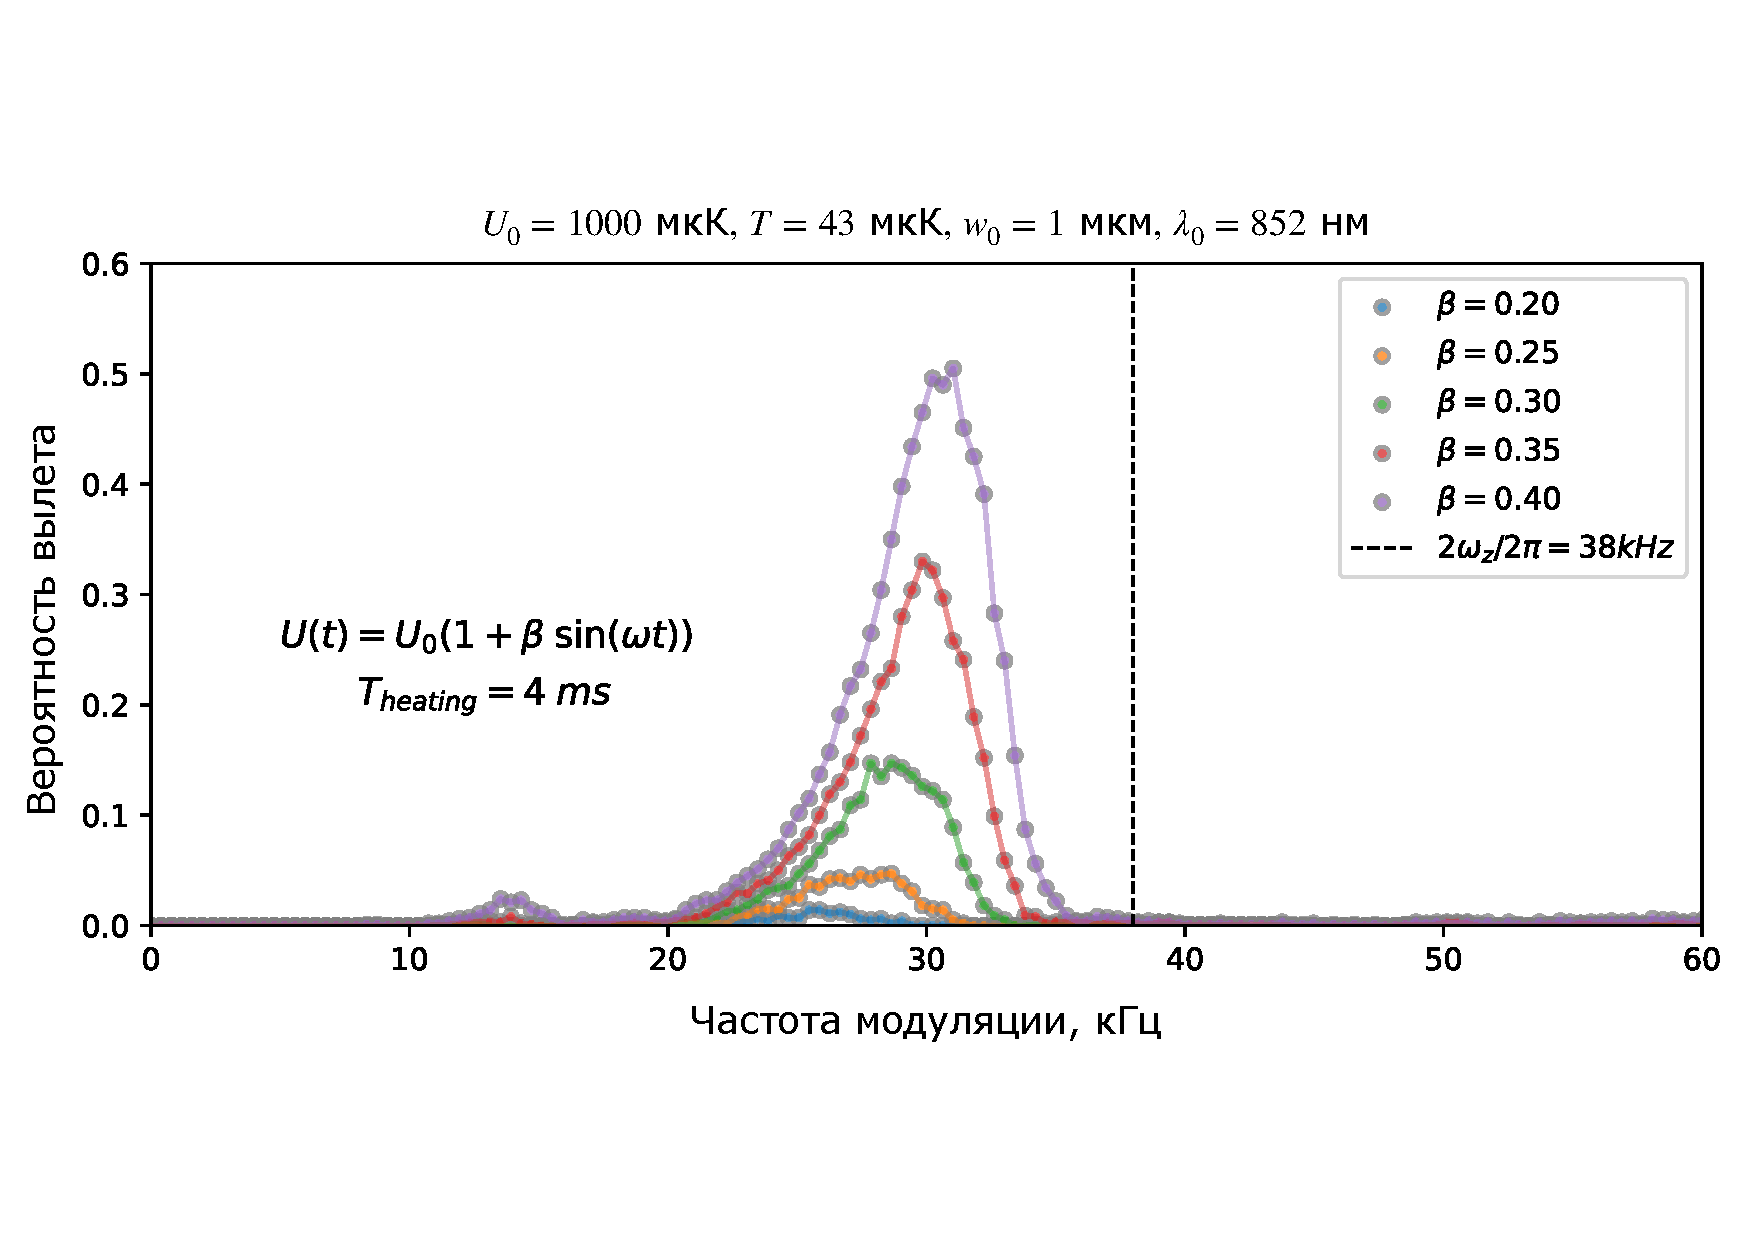
\includegraphics[width=0.8\textwidth]{images/parametric_test.pdf}
	\caption{Моделирование параметрического нагрева атома для немного других экспериментальных параметров. Центр резонанса сдвинут, форма линии асимметрична.}
	\label{fig:parametric_test}
\end{figure}

В процессе измерений также выяснилось, что важно начинать раскачку потенциала ловушки уже после загрузки атомов. Если запускать модуляцию глубины ловушки во время загрузки атомов, то резонансов в вероятности вылета атома не наблюдается. Скорее всего, это связано с тем, что атомы, которые могут вылететь из-за параметрической раскачки, просто не загружаются в ловушку. 

\subsubsection{Температура атома, эксперимент release and recapture}
\label{sec:atom_temp}

Температура атома измеряется стандартным способом по эксперименту release and recapture \cite{Tuchendler2008EnergyDA}. При выключении потенциала оптической ловушки атом удаляется от ловушки и, при достаточно большом времени выключения, вылетает. Измерения вероятности вылета от времени выключения аппроксимируются моделированием Монте-Карло, получается температура атома. Результаы измерения температуры атома показаны на рисунке \ref{fig:temperature}, температура атома в ловушке глубиной $700\text{ мкК}$ составила $40\text{ мкК}$.

\begin{figure}[H]
	\centering
	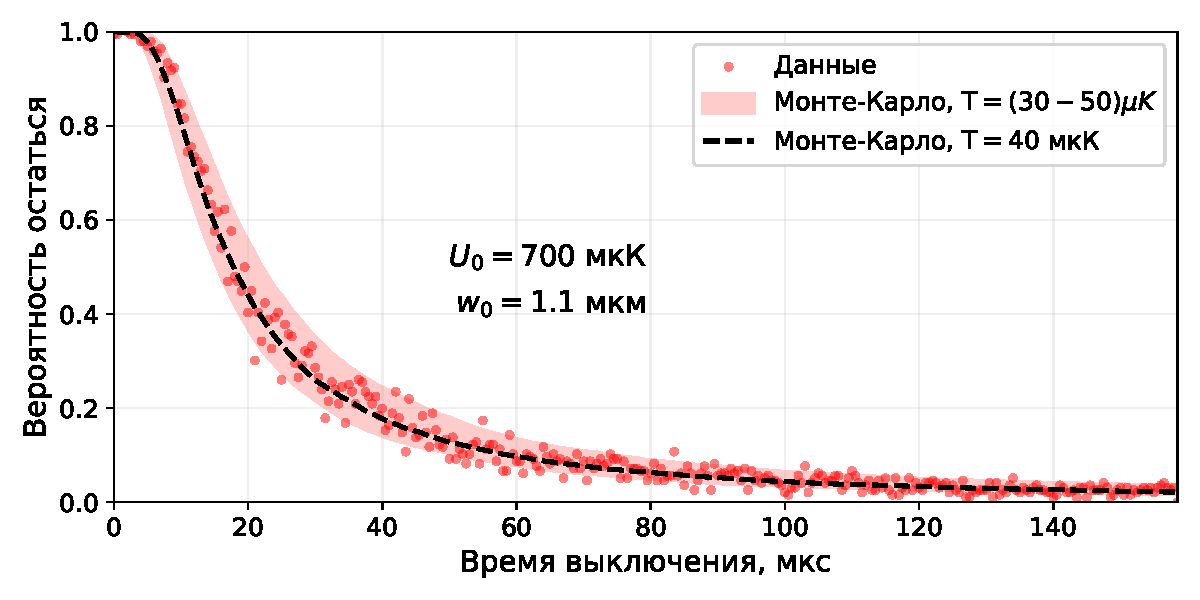
\includegraphics[width=0.6\textwidth]{images/temperature.pdf}
	\caption{Измерение температуры атома с помощью метода release and recapture. Аппроксимация с помощью Монте-Карло.}
	\label{fig:temperature}
\end{figure}

Измерения температуры атома удобнее выполнять в глубокой ловушке, но при выполнении логических операций глубина ловушки адиабатически опускается \cite{Tuchendler2008EnergyDA} до ранее измеренного значения $U_0 = 340\text{ мкК}$. При адиабатическом опускании глубины ловушки сохраняется фазовый объём системы \cite{LL_mechanics}, то есть для нашей системы получаем $E_{x}/\omega_r = const, \; E_{y}/\omega_r = \text{const}, \; E_{z}/\omega_z = \text{const}$, так как колебания вдоль главных осей в гармоническом режиме можно рассматривать независимо, что можно переписать как $E/\sqrt{U_0} = \text{const}$ с учётом формул для колебательных частот $\omega_r, \omega_z \sim \sqrt{U_0}$. Также можно сказать, что адиабатическое опускание не меняет вероятности заселения уровней трёхмерного осциллятора. Пусть в начале атом с температурой $T_{1}$ сидит в ловушке глубиной $U_1$. После изменения глубины ловушки до $U_{2}$ температура атома поменяется на $T_{2}$, причем вероятности состояний не изменятся 

\begin{equation}
	\exp\left(-\frac{E_{1}}{kT_{1}}\right) = \exp\left(-\frac{E_{2}}{kT_{2}}\right) \Leftrightarrow \frac{E_{1}}{T_{1}} = \frac{E_{2}}{T_{2}}.
\end{equation}

С учётом адиабатического инварианта осциллятора $E/\sqrt{U_0} = \text{const}$ получаем соотношение между глубиной ловушки и температурой до и после адиабатического опускания в гармоническом режиме

\begin{equation}
	\frac{\sqrt{U_{1}}}{T_{1}} = \frac{\sqrt{U_{2}}}{T_{2}}.
\end{equation}

Отсюда для $U_{1} = 700\text{ мкК}, \; T_{1} = 40\text{ мкК}, \; U_{2} = 340\text{ мкК}$ получаем тепературу после адиабатического опускания $T_{2} = 30\text{ мкК}$. Окончательно получаем температуру $T = 30 \text{ мкК}$ при глубине ловушки $U_0 = 340\text{ мкК}$.

\subsubsection{Результаты моделирования}
\label{sec:raman_model_results}

Результаты моделирования и сравнение с экспериментом показаны на рисунке \ref{fig:ICQT_res}, точность однокубитной операции для $w_R = 6.0\text{ мкм}$ составила $F = (99.56 \pm 0.03)\%$ по результатам randomized benchmarking \cite{Hines_2023}. Было продемонстрировано существенное улучшение точности однокубитных операций за счёт увеличения размера пучка. Такой подход, однако, не подходит для реализации локальных рамановских операций, так как для выполнения двухкубитных операций атомы располагаются на расстоянии $3.4\text{ мкм}$, то есть при радиусе перетяжки рамановского лазера $6.0 \text{ мкм}$ основным источником ошибок будет кроссток. 

\begin{figure}[H]
	\centering
	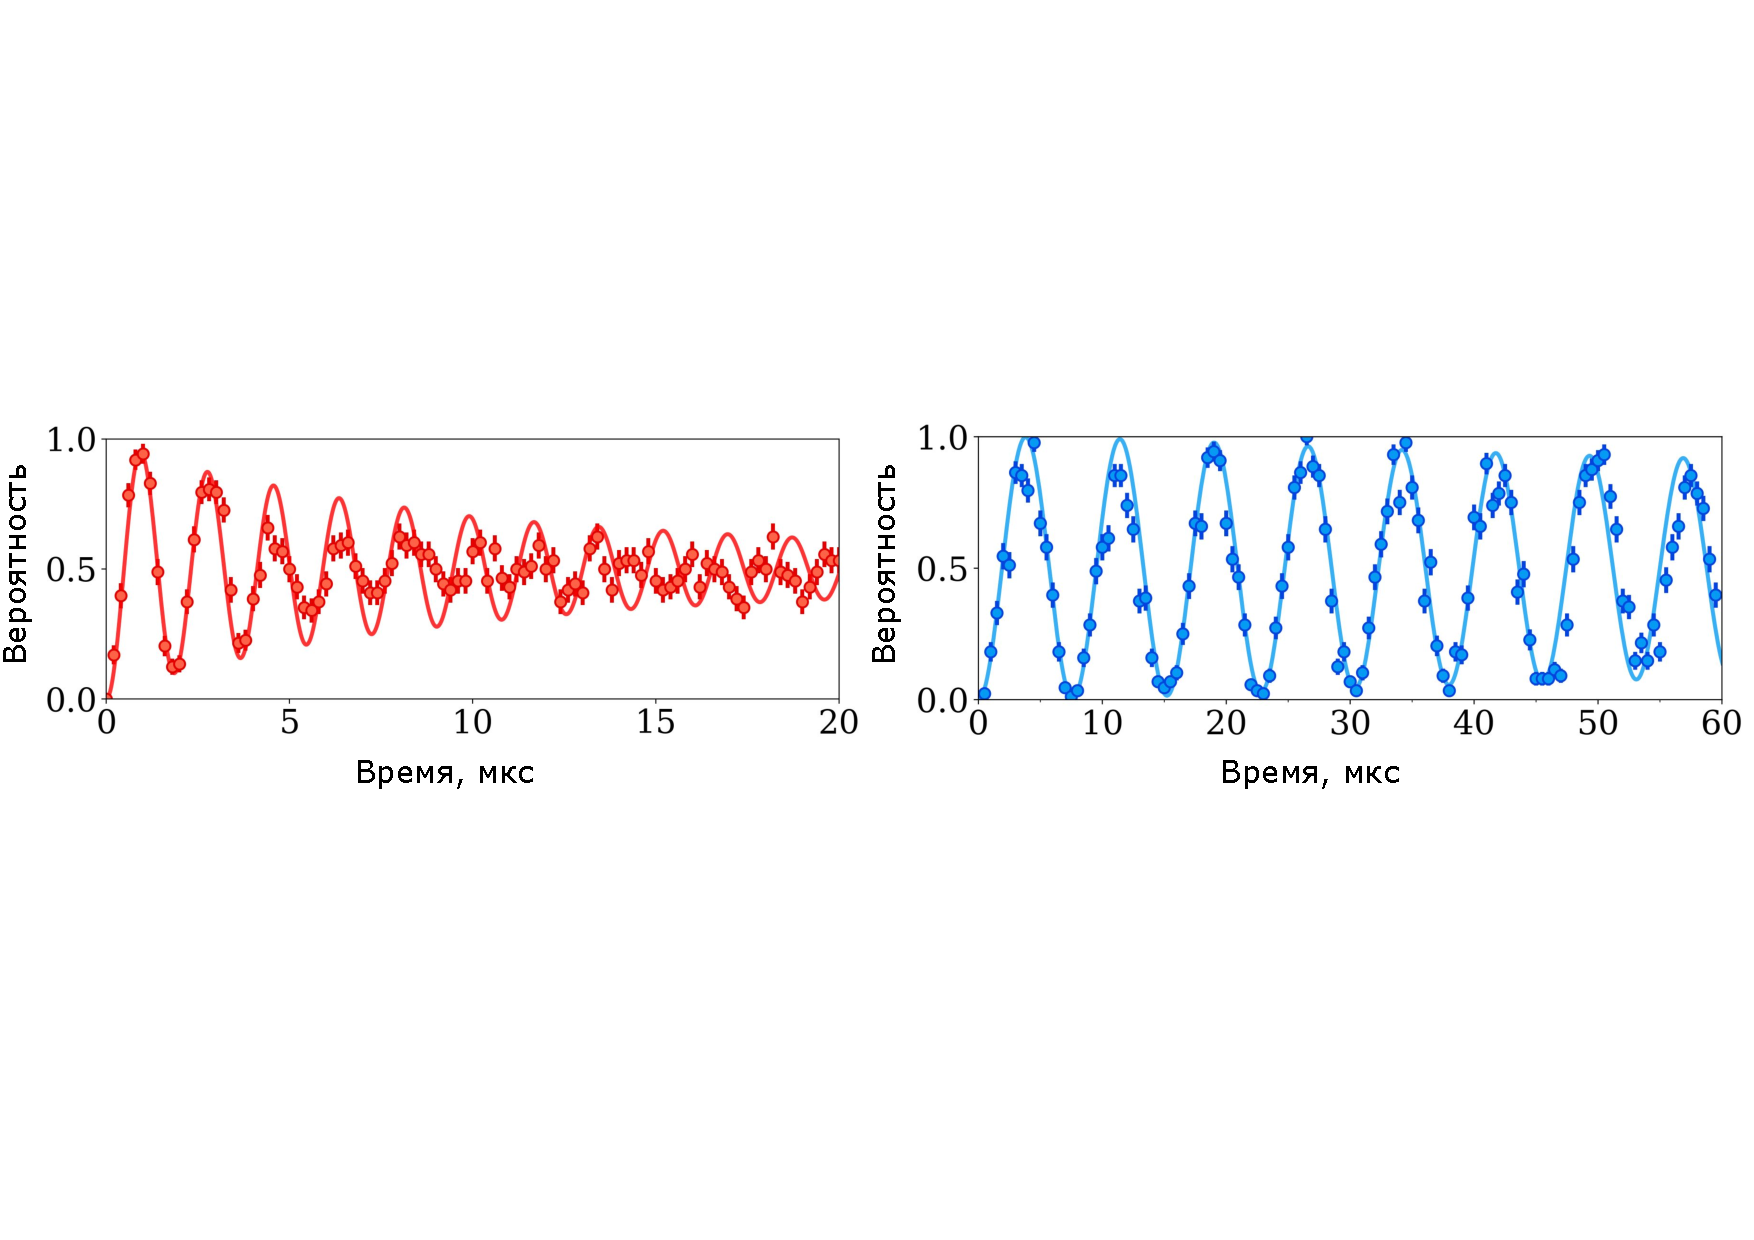
\includegraphics[width=1.0\textwidth]{images/raman_ICQT_res.pdf}
	\caption{Осцилляции Раби с рамановским двухфотонным возбуждением для $w_R = 2\text{ мкм}$ и $w_R=6.0 \text{ мкм}$}. 
	\label{fig:ICQT_res}
\end{figure}

% \subsection{Улучшение логических операций за счёт flat-top пучков}

\subsection{Импульсная последовательность BB1}

\subsubsection{Введение}

Одним из недостатков однокубитных вентилей на рамановских двухфотонных переходах является их сильная чувствительность к тепловому движению атома, амплитудным шумам лазера и неоднородностям интенсивности лазера по атомному массиву. Происходит это из-за того, что двухфотонная частота Раби, в отличие от однофотонной $\Omega \sim E$, пропорциональна уже произведению амплитуд ЭМ-полей возбуждающих лазеров $\Omega_R \sim E_1 E_2^*$. Так как в нашем случае оба ЭМ-поля создаются одним лазером за счёт модуляции интенсивности, то двухфотонная частота Раби пропорциональна интенсивности $\Omega \sim I$. Как было показано, вклад теплового движения атома можно компенсировать за счёт использования более широких возбуждающих пучков и пучков flat-top. При использовании более широких возбуждающих пучков возникает проблема с адресацией, так как засвечиваются сразу много атомов, а также снижается двухфотонная частота Раби при фиксированных отстройке от двухфотонного резонанса и интенсивности лазера. Работа с flat-top пучками затруднена тем, что они сильно чувствительны к аберрациям, особенно при жёсткой фокусировке на атом. Также оба подхода не решают проблему с чувствительностью к амплитудным шумам лазера и неоднородностью интенсивности по массиву. 


Альтернативой двум предложенным подходам является использование импульсных последовательностей устойчивых к отклонениям частоты Раби в качестве однокубитных гейтов. Например, можно взять импульсную последовательность BB1(BroadBand 1)\cite{Wimperis1994BroadbandNA,WIMPERIS1989509,WIMPERIS199046}, использовать её в качестве $X, Y$ - гейтов. Для реализации $Z$-гейтов последовательность BB1 использовать не требуется, так как они делаются при большой отстройке от резонанса, эти гейты не чувствительны к отклонениям частоты Раби. 

Рассмотрим импульсную последовательность вида

\begin{equation}
	\pi_{\phi_1} \pi_{\phi_2} \pi_{\phi_3} \pi_{\phi_4} \theta_0,
\end{equation}

где $\theta_\phi$ - поворот на сфере Блоха на угол $\theta$ вокруг оси $\vec{n}_\phi = \left(\cos \phi, \sin \phi, 0 \right)^T$. Такой импульсной последовательности соответствует унитарный оператор 

\begin{equation}
	U = \exp\left( - i \frac{\theta}{2} \sigma_x \right)\exp\left( - i \frac{\pi}{2} \sigma_{\phi_4}\right)\exp\left( - i \frac{\pi}{2} \sigma_{\phi_3}\right)\exp\left( - i \frac{\pi}{2} \sigma_{\phi_2}\right)\exp\left( - i \frac{\pi}{2} \sigma_{\phi_1}\right),
\end{equation}

где $\sigma_\phi = \sigma_x\cos \phi + \sigma_y\sin \phi$. Так как 

\begin{equation}
	\begin{aligned}
		& \exp\left(-i \frac{\pi}{2} \sigma_\phi \right) = \cos \frac{\pi}{2} \sigma_0 - i\sin \frac{\pi}{2} \sigma_\phi = -i\sigma_\phi ,\\
		& \exp\left( - i \frac{\pi}{2} \sigma_{\phi_i}\right)\exp\left( - i \frac{\pi}{2} \sigma_{\phi_j}\right) = (-i)^2 \sigma_{\phi_i} \sigma_{\phi_j} = - \exp\left(-i(\phi_i - \phi_j)\sigma_z \right),
	\end{aligned}
\end{equation}

то оператор сводится к виду

\begin{equation}
	U = \exp\left( - i \frac{\theta}{2} \sigma_x \right)\exp\left( i(\phi_1 - \phi_2 +\phi_3 - \phi_4) \sigma_z\right).
\end{equation} 

Таким образом, чтобы реализовать вращение $\theta_0$ на сфере Блоха, нужно 

\begin{equation}
	\phi_1 - \phi_2 +\phi_3 - \phi_4 = 0.
\end{equation}

Физически поворот на сфере Блоха вокруг осей $X, Y$ соответсвует резонансным осцилляциям Раби в течение некоторого времени $\theta = \Omega t$. Пусть теперь частота Раби отклонилась от предполагаемого значения $\tilde{\Omega} = \beta \Omega$, то есть $\tilde{\theta} = \beta \theta$. Попробуем подобрать углы $\phi_i$ так, чтобы минимизировать влияние отклонения частоты Раби от идеального значения на точность операции. Унитарный оператор с учётом отклонения частоты примет вид


\begin{equation}
	U(\beta) = \exp\left( - i\beta \frac{\theta}{2} \sigma_x \right)\exp\left( - i \beta \frac{\pi}{2} \sigma_{\phi_4}\right)\exp\left( - i \beta \frac{\pi}{2} \sigma_{\phi_3}\right)\exp\left( - i \beta \frac{\pi}{2} \sigma_{\phi_2}\right)\exp\left( - i \beta \frac{\pi}{2} \sigma_{\phi_1}\right).
\end{equation}

Далее нам хочется получить малый параметр, здесь это отклонение частоты Раби от идеальной, т.е. $\delta = \beta - 1$. Попробуем перегруппировать множители так, чтобы прийти к виду

\begin{equation}
	U(\beta) = U_0 \tilde{U}(\delta),
\end{equation}

где $U_0$ - нужное нам вращение на сфере Блоха, $\tilde{U} \simeq \hat{1}$ при $\delta \sim 0$. Если привести оператор к такому виду, то как раз получится устойчивость импульсной последовательности к отклонениям частоты Раби. 


\begin{equation}
	\begin{aligned}
		& \exp\left( - i \beta \frac{\pi}{2} \sigma_{\phi_2}\right)\exp\left( - i \beta \frac{\pi}{2} \sigma_{\phi_1}\right) =&\\
		&= \exp\left( - i \frac{\pi}{2} \sigma_{\phi_2}\right)\exp\left(- i \frac{\pi}{2} \sigma_{\phi_1}\right)
		\begingroup\color{blue} \exp\left( i \frac{\pi}{2} \sigma_{\phi_1}\right)\exp\left( - i \delta \frac{\pi}{2} \sigma_{\phi_2}\right)\exp\left( - i \frac{\pi}{2} \sigma_{\phi_1}\right) \endgroup
		\exp\left( - i \delta \frac{\pi}{2} \sigma_{\phi_1}\right) =\\
		&= \exp\left( - i \frac{\pi}{2} \sigma_{\phi_2}\right)\exp\left(- i \frac{\pi}{2} \sigma_{\phi_1}\right)
		\begingroup\color{blue}\exp\left( - i \delta \frac{\pi}{2} \sigma_{\phi_2'}\right)\endgroup
		\exp\left( - i \delta \frac{\pi}{2} \sigma_{\phi_1}\right) 
	\end{aligned}
\end{equation}

Здесь выделенные вращения можно свести к одному вращению вокруг оси $\vec{n}_{\phi_2'}$, где $\phi_2' = - \phi_2 + 2\phi_1$. Обкладки вращения вокруг оси $\vec{n}_{\phi_2}$ соответсвуют замене базиса ($\tilde{A} = U^{\dagger}A U$), т.е. вектор $\vec{n}_{\phi_2}$ поворачивается вокруг $\vec{n}_{\phi_1}$ на угол $\pi$. Проще всего это понять, нарисовав на сфере Блоха. Действуя аналогичным образом, можно свести оператор к виду

\begin{equation}
\begin{aligned}
	U &= \exp\left( - i \frac{\theta}{2} \sigma_x \right)
	\begingroup\color{red}\exp\left( - i \frac{\pi}{2} \sigma_{\phi_4}\right)\exp\left( - i \frac{\pi}{2} \sigma_{\phi_3}\right)\exp\left( - i \frac{\pi}{2} \sigma_{\phi_2}\right)\exp\left( - i \frac{\pi}{2} \sigma_{\phi_1}\right)\endgroup \times &\\
	&\times \begingroup\color{blue}\exp\left( - i\delta \frac{\theta}{2} \sigma_x \right)\exp\left( - i \delta \frac{\pi}{2} \sigma_{\phi_4'}\right)\exp\left( - i \delta \frac{\pi}{2} \sigma_{\phi_3'}\right)\exp\left( - i \delta \frac{\pi}{2} \sigma_{\phi_2'}\right)\exp\left( - i \delta \frac{\pi}{2} \sigma_{\phi_1'}\right)\endgroup =& \\
	&= \exp\left( - i \frac{\theta}{2} \sigma_x \right)\begingroup\color{blue}\exp\left( - i \delta \frac{\theta}{2} \sigma_x \right)\endgroup\begingroup\color{red}\exp\left(i(\phi_1 - \phi_2 + \phi_3 - \phi_4)\sigma_z\right)\endgroup \times & \\
	&\times \begingroup\color{blue}\exp\left( - i\delta \frac{\theta}{2} \sigma_x \right)\exp\left( - i \delta \frac{\pi}{2} \sigma_{\phi_4'}\right)\exp\left( - i \delta \frac{\pi}{2} \sigma_{\phi_3'}\right)\exp\left( - i \delta \frac{\pi}{2} \sigma_{\phi_2'}\right)\exp\left( - i \delta \frac{\pi}{2} \sigma_{\phi_1'}\right)\endgroup =&\\
	&= \exp\left( - i \frac{\theta}{2} \sigma_x \right) \begingroup\color{blue}\tilde{U}(\delta)\endgroup,
\end{aligned}
\end{equation}

где углы $\phi_i'$ задаются формулой 
\begin{equation}
	\phi_j' = (-1)^{j-1}\phi_j + 2\sum_{k=1}^{j-1}(-1)^{k-1}\phi_k.
\end{equation}


В случае $\delta = 0$ кроме нужного нам вращения также совершается дополнительное вращение вокруг оси $z$. Чтобы его исключить, потребуем $\phi_1 - \phi_2 + \phi_3 - \phi_4 = 0$. Также благодаря этому можно собрать все помеченные синим цветом слагаемые рядом. С помощью формулы Бейкера-Кэмпбелла-Хаусдорфа $\exp{X} \exp{Y} = \exp{\left(X + Y + \frac{1}{2}\left[X, Y \right] + \ldots\right)}$ соберём множители $\tilde{U}(\delta)$ в одну матричную экспоненту, сгруппировав слагаемые одного порядка малости по $\delta$. Получим

\begin{equation}
	\tilde{U}(\delta) = \exp{\left\{ -i\delta \frac{\pi}{2}\left(\frac{\theta}{\pi}\sigma_x + \sum_{i=1}^{4}\sigma_{\phi_i'} \right) - \delta^2 \frac{\pi^2}{8}\left(\frac{\theta}{\pi}\sum_{i=1}^{4}[\sigma_x,\sigma_{\phi_i'}]+
	\sum_{i=1}^{4} \sum_{j<i} \left[\sigma_{\phi_i'},\sigma_{\phi_j'}\right]\right)+\ldots \right\}}.
\end{equation}

После упрощений получается

\begin{equation}
	\tilde{U}(\delta) = \exp{\left\{ -i\delta \Phi_1 - i\delta^2 \Phi_2+\ldots \right\}},
\end{equation}
где операторы $\Phi_1$ и $\Phi_2$ определяются как

\begin{equation}
	\begin{aligned}
		\Phi_1 & = \frac{\pi}{2}\left(\sigma_x \left(\frac{\theta}{\pi} + \sum_{i=1}^{4}\cos \phi_i' \right)+\sigma_y \sum_{i=1}^{4}\sin \phi_i'\right), \\
		\Phi_2 & = \frac{\pi^2}{4}\sigma_z\left(\frac{\theta}{\pi}\sum_{i=1}^{4}\sin \phi_i' + 
	\sum_{i=1}^{4} \sum_{j<i} \sin\left(\phi_i' - \phi_j'\right) \right).
	\end{aligned}
\end{equation}

Таким образом, получается следующая система уравнений на углы $\phi_i$

\begin{equation}
	\begin{cases}
		\phi_i' = (-1)^{i-1} \phi_i + 2 \sum_{j=1}^{i-1}(-1)^{j-1}\phi_j \\
		\sum_{i=1}^{4} (-1)^i \phi_i' = -\sum_{i=1}^{4} (-1)^i \phi_i = 0 \\
		\sum_{i=1}^{4} \sin \phi_i' = 0 \\ 
		\frac{\theta}{\pi} + \sum_{i=1}^{4} \cos \phi_i' = 0 \\ 
		\frac{\theta}{\pi}\sum_{i=1}^{4}\sin \phi_i' + 
	\sum_{i=1}^{4} \sum_{j<i} \sin\left(\phi_i' - \phi_j'\right) = 0, \;\;\; \text{для зануления вклада с $\delta^2$}
	\end{cases}
\end{equation}


Решение такой системы неоднозначно, но можно искать его в виде $\phi_1 = \phi_4, \; \phi_2 = \phi_3$, тогда автоматически выполняются условия $\phi_1-\phi_2+\phi_3-\phi_4=0, \;\; \sum_{i=1}^{4}\sum_{j<i}\sin\left(\phi_i'-\phi_j'\right)=0$, а сама система приводится к виду

\begin{equation}
	\begin{cases}
		\phi_1 = \phi_4, \; \phi_2 = \phi_3 \\
		\phi_1' = \phi_4' = \phi_1\\
		\phi_2' = \phi_3' = -\phi_2 + 2\phi_1\\
		\sin \phi_1' + \sin \phi_2' = 0 \\ 
		\frac{\theta}{2\pi} + \cos \phi_1' + \cos \phi_2' = 0 \\ 
	\end{cases}
\end{equation}

Видно, что в качестве решения можно взять $\phi_1' = -\phi_2' = \phi$, $\phi = \arccos\left( -\frac{\theta}{4\pi}\right)$. В итоге получится импульсная последовательность BB1 \cite{Wimperis1994BroadbandNA, WIMPERIS199046,WIMPERIS1989509} устойчивая к отклонениям частоты Раби.

\begin{equation}
	\text{BB1:} \;\;\;  \pi_\phi \; 2\pi_{3\phi} \; \pi_\phi \; \theta_0, \;\;\; \phi = \arccos\left( -\frac{\theta}{4\pi}\right).
\end{equation}

То же самое можно проделать для вращения вокруг произвольной оси в плоскости $xy$ под углом $\xi$ к орту $x$, получится более общий вид последовательности

\begin{equation}
	\text{BB1:} \;\;\;  \pi_{\phi+\xi} \; 2\pi_{3\phi+\xi} \; \pi_{\phi+\xi} \; \theta_\xi, \;\;\; \phi = \arccos\left( -\frac{\theta}{4\pi}\right).
\end{equation}

В частности можно привести выражения для $X$ и $Y$ гейтов

\begin{equation}
	\begin{aligned}
		& \text{BB1-X:} \;\;\;  \pi_{\phi} \; 2\pi_{3\phi} \; \pi_\phi \; \pi_0,  \\
		& \text{BB1-Y:} \;\;\;  \pi_{\phi+90^{\circ}} \; 2\pi_{3\phi + 90^\circ} \; \pi_{\phi+ 90^\circ} \; \pi_{90^\circ}, \\ 
		& \phi = 104.478 ^\circ
	\end{aligned}
\end{equation}


\begin{figure}[tb]
	\centering
	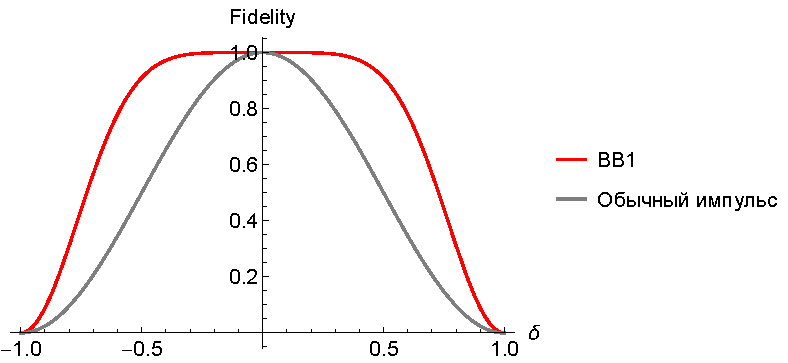
\includegraphics[width=0.48\textwidth]{images/fidelity_BB1.pdf}
	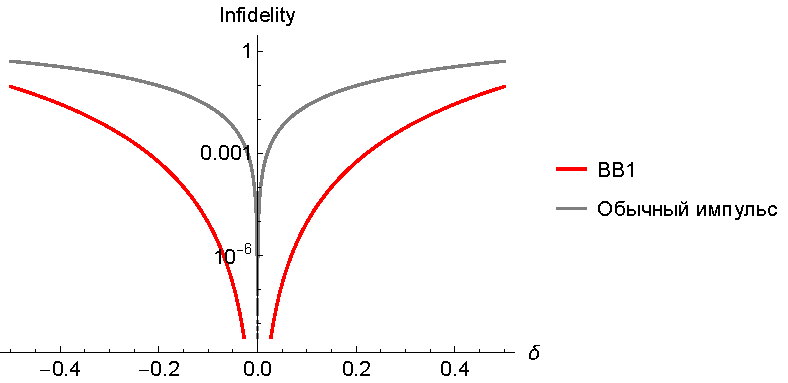
\includegraphics[width=0.48\textwidth]{images/infidelity_BB1.pdf}
	\caption{Зависимость точности $X,Y$ гейтов от отклонения частоты Раби.}
	\label{fig:BB1}
\end{figure}

\begin{figure}[tb]
	\centering
	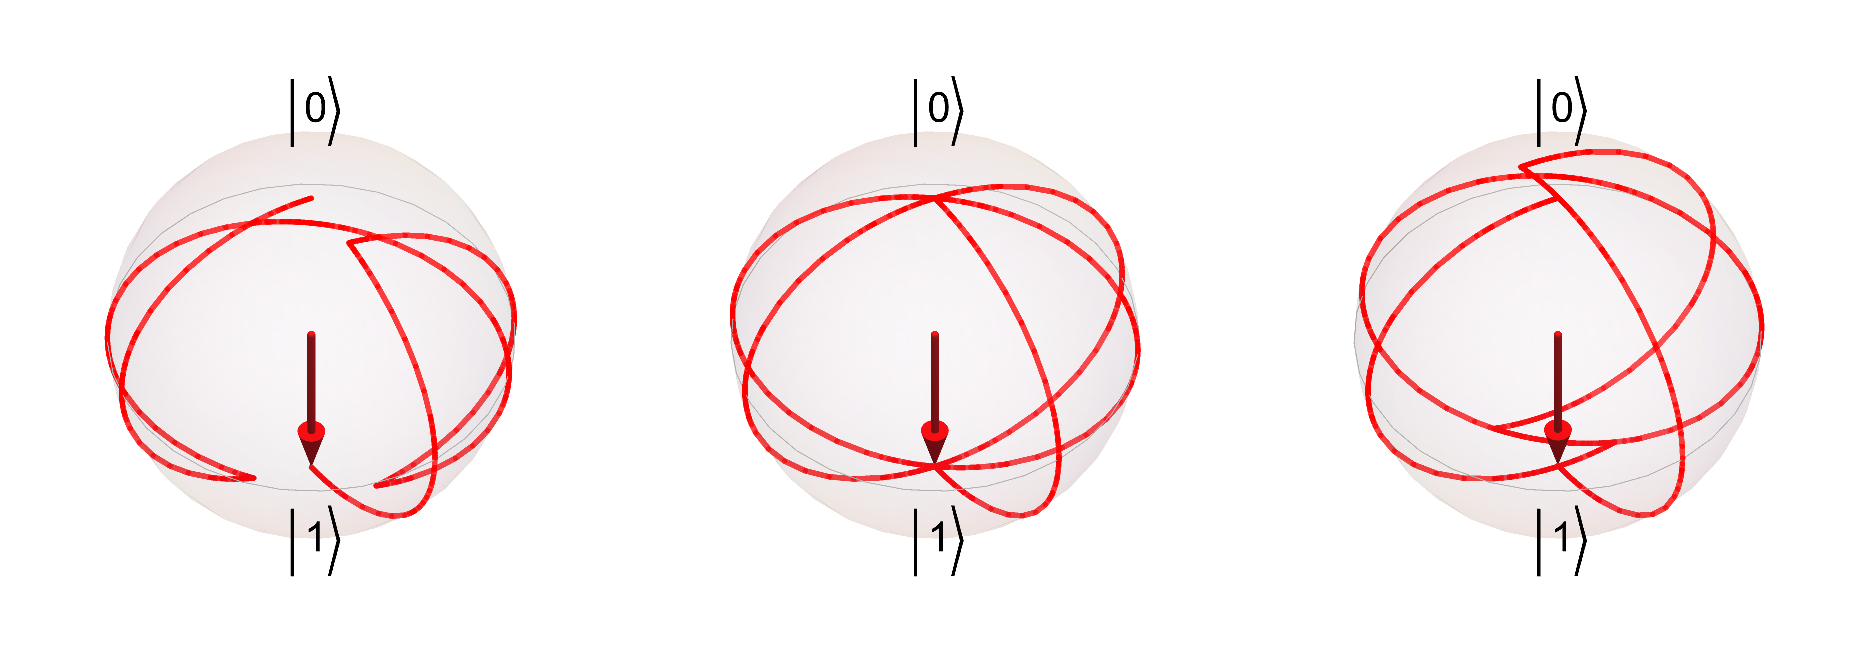
\includegraphics[width=1.0\textwidth]{images/BB1_Paths.pdf}
	\caption{Слева направо: траектории кубита в начальном состоянии $\ket{0}$ под действием импульса BB1X для $\beta=0.9, \; 1.0, \; 1.1.$}
	\label{fig:BB1}
\end{figure}

Так как амплитудные шумы лазера и тепловое движение атома достаточно медленные по сравнению с частотой Раби, то их можно рассматривать просто как отклонения частоты Раби, не зависящие от времени. Неоднородности интенсивности по массиву также не зависят от времени, определяются эффективностью работы АОД для разных углов отклонения. Таким образом, использование BB1-импульсов позволяет побороть сразу несколько проблем для рамановских гейтов. Можно на это возразить, что при использовании последовательности возрастает время однокубитной операции, таким образом усиливается время спонтанного распада из промежуточного состояния, а также влияние других механизмов декогеренции, однако использование последовательности BB1 позволяет работать при ширине перетяжки возбуждающих пучков, близких к ширине перетяжки оптического пинцета. Это позволяет делать локальные однокубитные операции, а также фокусировать большую интенсивность на атом и увеличивать отстройку от промежуточного уровня. Также последовательность BB1 полезна для радиочастотных гейтов в целях компенсации неоднородности излучения СВЧ-антенны. Более общий метод построения последовательностей такого типа, а также некоторые другие импульсные последовательности можно найти, например, в статьях \cite{PhysRevA.83.053420,Chuang_Composite}.

\subsubsection{Моделирование}

Как было показано, импульсная последовательность BB1 устойчива к отклонениям частоты Раби, то есть потенциально устойчива к тепловому движению атома, амплитудным шумам лазера, неоднородностям интенсивности лазера по атомному массиву. Однако, все полученные выкладки были сделаны в предположении, что частота Раби не зависит от времени, а просто смещена от идеального значения. Такое предположение работает, если тепловое движение одиночного атома в оптическом пинцете, а также амплитудные шумы лазера достаточно медленны по сравнению с двухфотонной частотой Раби для рамановских переходов. 

Также остаётся открытым вопрос о влиянии спонтанного распада с промежуточного состояния на точность однокубитных операций при использовании последовательности импульсов. За счёт увеличения длительности однокубитного гейта может оказаться так, что весь выигрыш от использования последовательности импульсов теряется из-за спонтанного распада из промежуточного состояния. Для исследования этих вопросов проведём численное моделирование возбуждения одиночного атома в оптическом пинцете с учётом теплового движения, кросстока между соседними кубитами и спонтанного распада из промежуточного состояния для последовательности BB1. По аналогии с \ref{sec:spontaneous} ошибку из-за спонтанного распада для $\pi$-импульса BB1 можно оценить как

\begin{equation}
	\left(1-F\right)_{sp}=\frac{5}{2}\frac{R}{\Omega_R}=\frac{\Gamma}{4\Delta},	
\end{equation}

Для $\Delta=2\pi\times 50 \text{ ГГц},\; \Gamma=2\pi \times 6 \text{ MГц}$ получаем ошибку из-за спонтанного распада для импульса BB1 $\left(1-F\right)_{sp} = 1.5\times{10}^{-4}$. Результаты моделирования с учётом теплового движения атома, кросстока между соседними кубитами и спонтанного распада из промежуточного состояния показаны на рисунке \ref{fig:errors_pipulse_total}. Значение ошибки при оптимальном радиусе перетяжки рамановского лазера $w_R =1.5 \text{ мкм}$ для последовательности BB1 составляет $1.6 \cdot 10^{-4}$, что определяется ошибкой из-за спонтанного распада $1.5 \cdot 10^{-4}$. В части \ref{sec:raman_model_results} было показано, что для обычного импульса значение ошибки при оптимальном радиусе перетяжки $w_R = 2.0 \text{ мкм}$ составляет $3 \cdot 10^{-3}$

\begin{figure}[H]
	\centering
	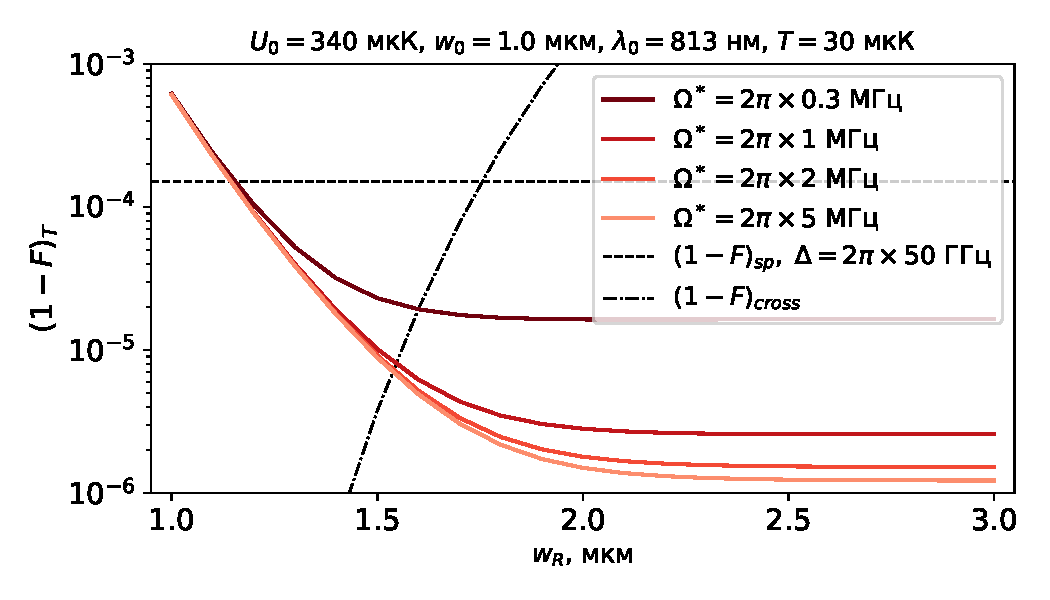
\includegraphics[width=0.48\textwidth]{images/BB1_Omega.pdf}
	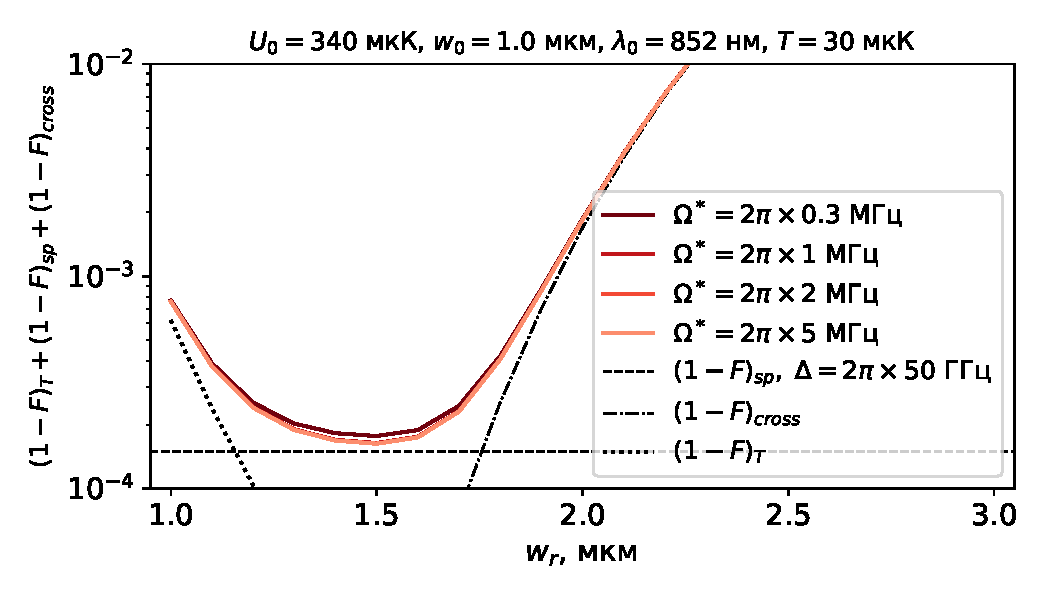
\includegraphics[width=0.48\textwidth]{images/BB1_Omega_total.pdf}
	\caption{Слева: ошибка из-за теплового движения для $\pi$-импульса BB1. Справа: суммарная ошибка из-за теплового движения, кросс-тока и спонтанного распада для $\pi$-импульса BB1.}
	\label{fig:errors_pipulse_total}
\end{figure}

На рисунке \ref{fig:BB1_offset_contor} приведены тепловые карты для ошибки обычного $\pi$-импульса и $\pi$-импульса BB1 от отстройки и отклонения частоты Раби. Для последовательности BB1 видна устойчивость к отклонениям частоты Раби в узком диапазоне отстроек от резонанса. Поведение зависимости \ref{fig:BB1} для разных значений отстроек от двухфотонного резонанса показано на рисунке  

\begin{figure}[H]
	\centering
	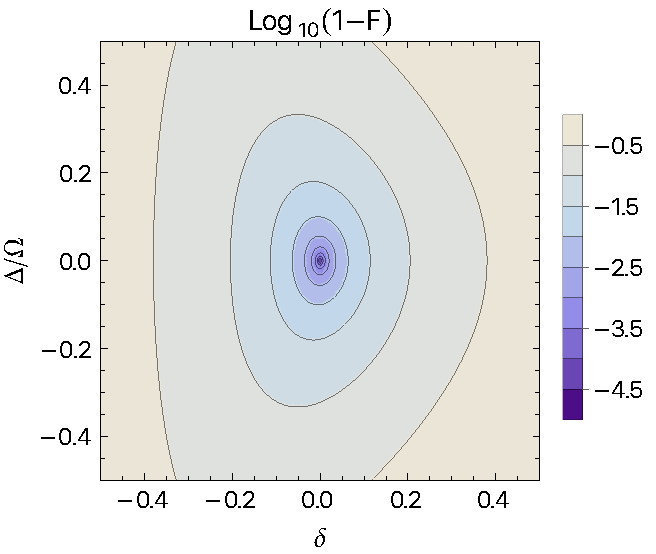
\includegraphics[width=0.4\textwidth]{images/pulse_offset_contor.pdf}
	\hspace{1em}
	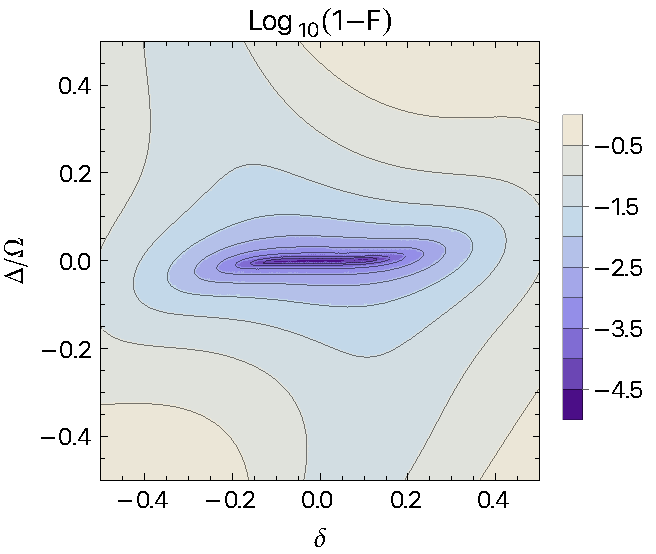
\includegraphics[width=0.4\textwidth]{images/BB1_offset_contor.pdf}
	\caption{Слева: зависимость ошибки обычного $\pi$-импульса от отстройки и отклонения частоты Раби. Справа: зависимость ошибки $\pi$-импульса BB1 от отстройки и отклонения частоты Раби.}
	\label{fig:BB1_offset_contor}
\end{figure}


\begin{figure}[H]
	\centering
	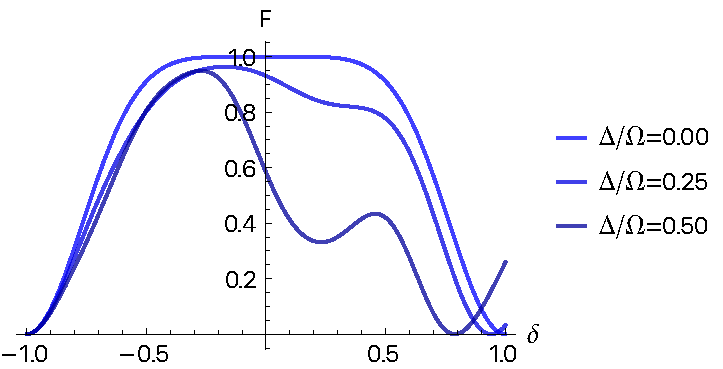
\includegraphics[width=0.5\textwidth]{images/BB1_offset.pdf}
	\caption{Искажение устойчивости последовательности BB1 при ненулевой отстройке от резонанса.}
	\label{fig:BB1_offset}
\end{figure}

\subsubsection{Эксперимент}

Для экспериментальной реализации последовательности импульсов BB1 требуется модулировать фазу рамановского лазера, то есть получить фазовый множитель в двухфотонной частоте Раби $\Omega_R e^{i\phi\left(t\right)}$. Это можно сделать, например, с помощью IQ-модуляции сигнала, подающегося на модулятор интенсивности. Принципиальная схема установки показана на рисунке \ref{fig:IQ_modulation}. В IQ-модулятор подаются два сигнала вида $I\left(t\right)=\sin\left(\omega t+\phi\left(t\right)\right), Q\left(t\right)=\cos\left(\omega t+\phi\left(t\right)\right)$, которые затем перемножаются с сигналом несущей $\cos\left(\omega_ct\right), \;  \sin\left(\omega_ct\right)$ и суммируются. В результате получается сигнал $S\left(t\right)=I\left(t\right)\cos\left(\omega_ct\right)+Q\left(t\right)\sin\left(\omega_ct\right)=\sin\left(\left(\omega_c+\omega\right)t+\phi\left(t\right)\right)$, который подаётся на модулятор интенсивности. Модулятор интенсивности далее создаёт рамановский лазер с фазовой модуляцией $\Omega_R e^{i\phi\left(t\right)}$. Для генерации I/Q -компонент используется плата Red Pitaya STEMlab 125-14 со встроенным генератором сигналов произвольной формы. После подачи внешнего триггера на порт DIO\_0P (EXT TRIG.) начинается воспроизведение I/Q – компонент с аналоговых выходов OUT1, OUT2, которые далее подаются на IQ – модулятор. 


\begin{figure}[H]
 	\centering
 	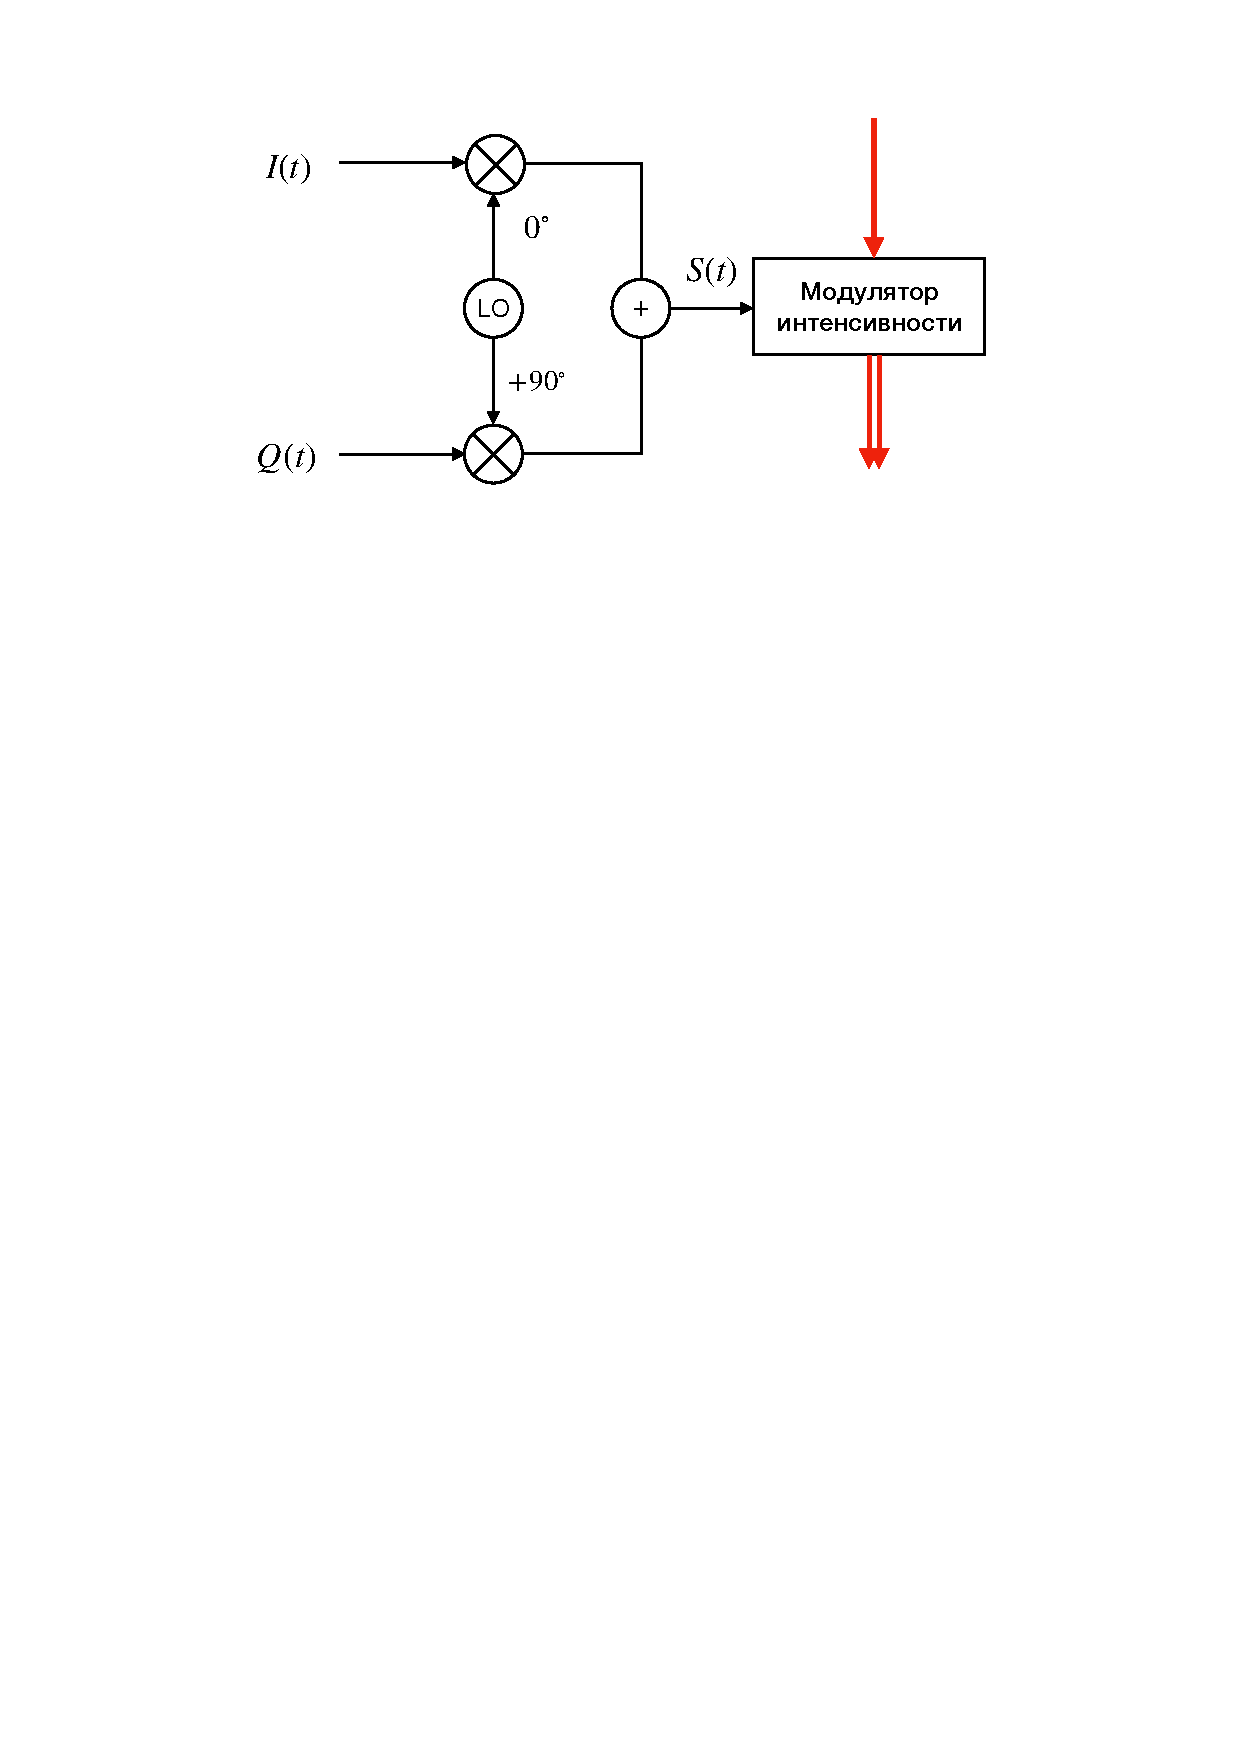
\includegraphics[width=0.7\textwidth]{images/IQ_modulation.pdf}
 	\caption{Сигналы $I(t)$ и $Q(t)$, содержащие фазовую модуляцию, смешиваются с сигналом несущей (LO), получается требуемый сигнал модуляции $S(t)$, который подаётся на модулятора интенсивности.}
 	\label{fig:IQ_modulation}
\end{figure} 

I/Q-компоненты также содержат несущую частоту $\omega$, это требуется так как использующийся I/Q-модулятор не пропускает постоянный сигнал. Так как суммарная частота сигнала после IQ-модулятора $\omega + \omega_c$ задаёт разность частот между компонентами рамановского лазера $2(\omega + \omega_c) \simeq 6.8 \text{ ГГц}$, требуется экспериментально подобрать резонансное значение частоты $\omega$ при фиксированной частоте $\omega_c$. Зависимость вероятности возбуждения после обычного рамановского $\pi$-импульса от частоты $\omega$ показана на рисунке \ref{fig:omega_scan}, по резонансу определяется требуемая частота модуляции $\omega$. 

\begin{figure}[H]
	\centering
	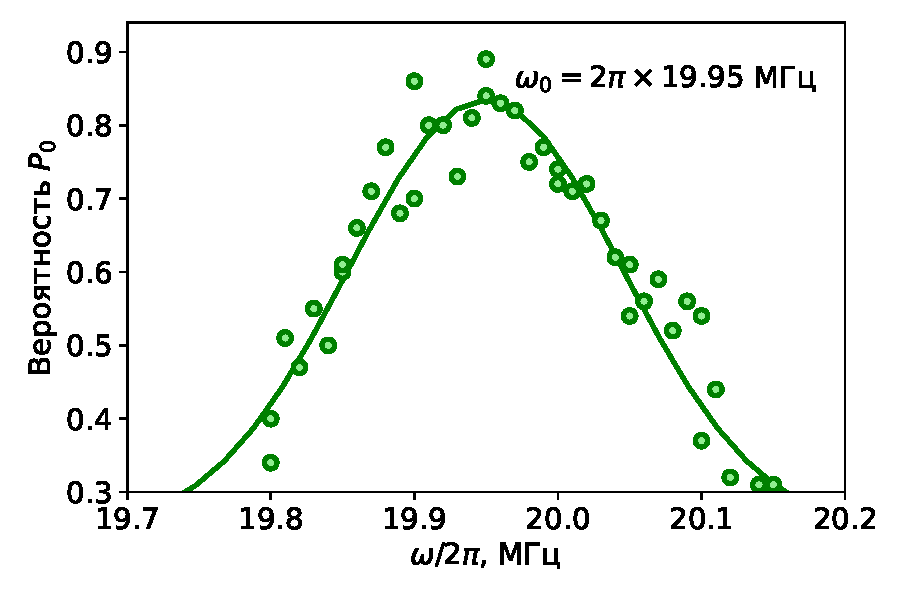
\includegraphics[width=0.7\textwidth]{images/omega_scan.pdf}
	\caption{По резонансу в вероятности возбуждения от частоты модуляции экспериментально определятся нужная частота модуляции.}
	\label{fig:omega_scan}
\end{figure}

После подбора правильной частоты модуляции были сняты зависимости осцилляций Раби с использованием последовательности BB1 (рис. ). Сканирование проводится в диапазоне $\theta \in (-2\pi, 2\pi)$, так как для большего угла поворота требуется отправлять с платы несколько импульсов BB1 подряд, это пока что не реализовано. Следует обратить внимание, что угол поворота $\theta$ на сфере Блоха задаёт как длительность последовательности $\Omega_R T_{BB1}(\theta) = 4\pi + \theta$, так и углы в фазовой модуляции $\phi(\theta) = \arccos(-\theta/4\pi)$. Для задания длительности импульса $T_{BB1}(\theta)$ на плате Red Pitaya так же требуется знать двухфотонную частоту Раби. Она определяется с помощью обычных осцилляций Раби с рамановским возбуждением с использованием платы Red Pitaya и триггера с внешнего генератора.

\begin{figure}[H]
	\centering
	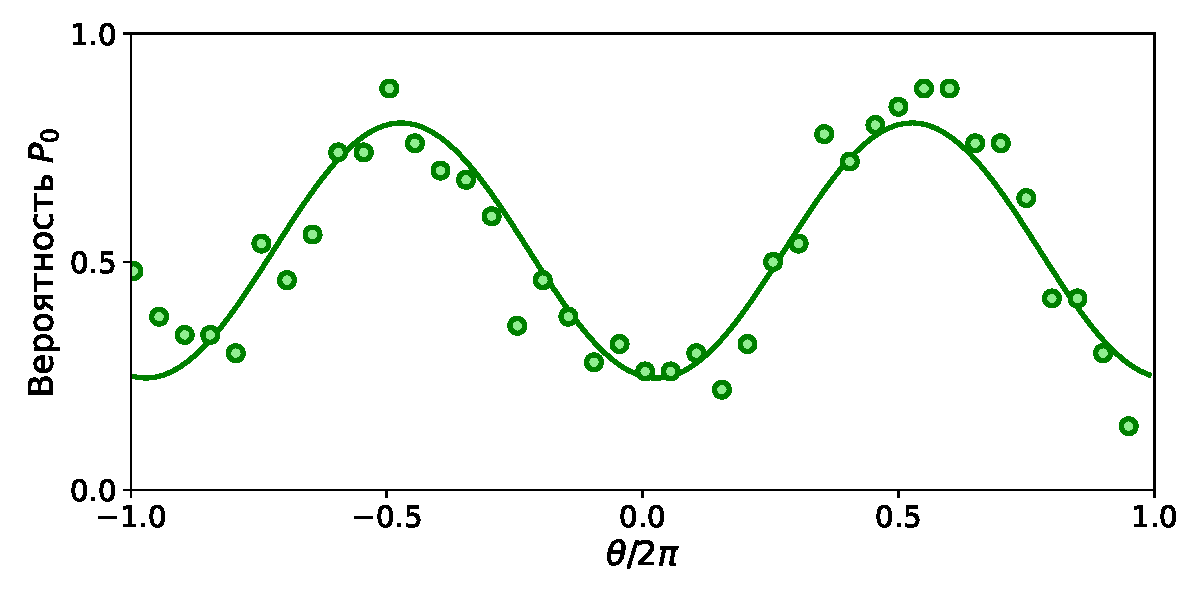
\includegraphics[width=0.7\textwidth]{images/theta_scan.pdf}
	\caption{Период сцилляций Раби с использованием последовательности BB1.}
	\label{fig:theta_scan}
\end{figure}

Также была снята зависимость вероятности возбуждения от суммарной длительности $\pi$-импульса $T_{BB1}(\pi)$, она показана на рисунке . Теоретически это эквивалентно сканированию частоты Раби, то есть ожидается зависимость как на рисунке \ref{fig:BB1}.

\begin{figure}[H]
	\centering
	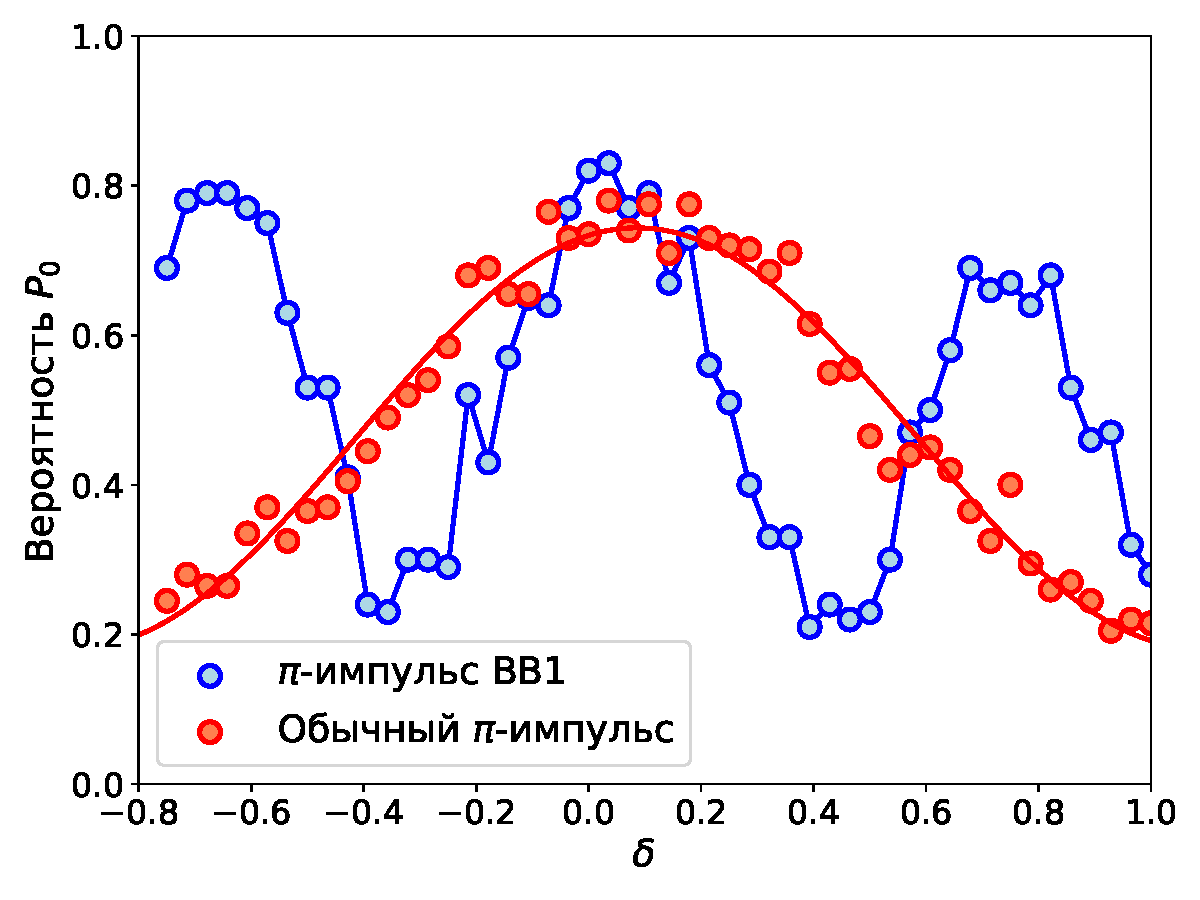
\includegraphics[width=0.48\textwidth]{images/delta_scan.pdf}
	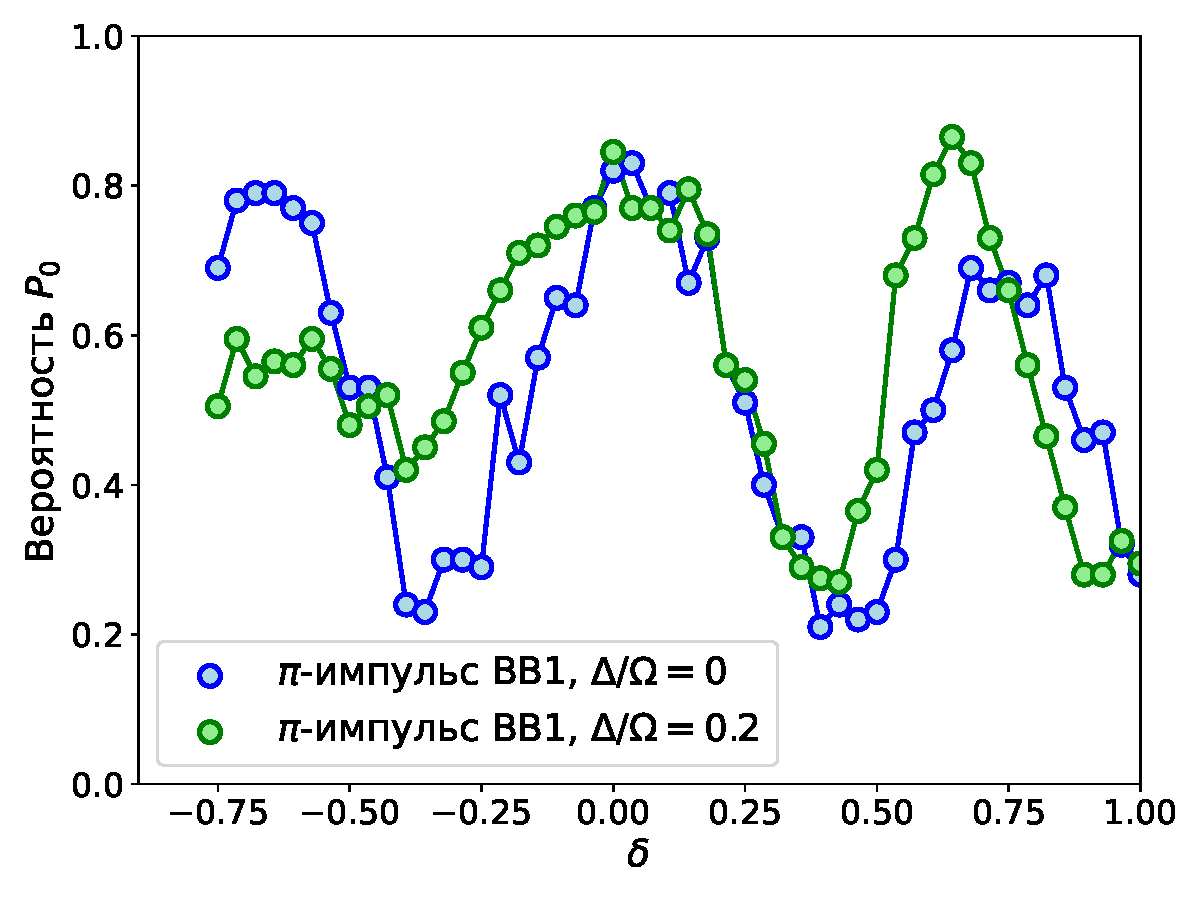
\includegraphics[width=0.48\textwidth]{images/delta_scan_offset.pdf}
	\caption{Слева: сканирование длительности $\pi$-импульса для обычного рамановского возбуждения и последовательности BB1, ожидалась зависимость как на рисунке \ref{fig:BB1}. Справа: при ненулевой отстройке от резонанса наблюдалась асимметричная зависимость, схожая по форме с \ref{fig:BB1_offset}.}
	\label{fig:BB1_experiment}
\end{figure}

Пока что не понятно почему наблюдается такая зависимость. При неправильной частоте модуляции $\omega$ наблюдалось асимметричное поведение ``устойчивости'' последовательности BB1, похожее на зависимость \ref{fig:BB1_offset}. После подбора правильной частоты модуляции (рис. \ref{fig:omega_scan}) это предположение отпало. Планируется дальнейшая работа в этом направлении.

\subsection{Результаты главы}

В этой части работы, посвященной улучшению точности однокубитных операций с рамановским двухфотонным возбуждением, получилось достичь следующих результатов:

\begin{enumerate}
	\item Определен основной источник ошибок в однокубитных операциях с двухфотонным рамановским возбуждением - тепловое движение атома в оптическом пинцете.
	\item Сделана численная модель, учитывающая тепловое движение атома, спонтанный распад из промежуточного состояния и кроссток между соседними атомами. Измерены параметры модели, настроен эксперимент по параметрическому нагреву атома, который ранее не работал.
	\item Исследована возможность применения пучков flat-top для локальных однокубитных операций. За счёт сильной чувствительности к аберрациям при жёсткой фокусировке на атом такой подход не кажется масштабируемым. Однако, использование таких пучков хорошо работает для двухкубитных операций, про это будет рассказано в следующей главе.
	\item Предложено использование последовательности BB1 для компенсации теплового движения атома, амплитудных шумов рамановского лазера и неоднородности интенсивности рамановского лазера, возникающей из-за разной эффективности дифракции АОД при адрессации на разные узлы атомного массива. 
	\item Проведено численное моделирование с учётом вышеперечисленных ошибок, последовательность оказалась устойчивой к тепловому движению атома. Это важный результат, так как последовательность BB1 изначально предназначена для компенсации статических отклонений частоты Раби от идеального значения. Было показано, что устойчивость также сохраняется при движении атома. Настроена экспериментальная схема для реализации последовательности BB1, начаты измерения.
\end{enumerate}

\newpage